\documentclass[10pt,letterpaper]{article}
\usepackage{graphicx}
\graphicspath{ {../png_images/} }

\usepackage{cogsci}
\usepackage{pslatex}
\usepackage{apacite}
\usepackage{makecell}
\usepackage{url}
\usepackage{graphicx}

\title{CANLab2024: A multiscale probabilistic meta-atlas of the healthy human brain}
 
\author{{\large \bf Bogdan Petre (bogdan.petre.gr@dartmouth.edu)} \\
  Department of Psychological and Brain Sciences, Dartmouth College \\
  3 Maynard Street, Hanover, NH 03755 USA
\AND {\large \bf Martin A Lindquist (mlindqui@jhsph.edu)} \\
  Department of Biostatistics, Johns Hopkins University \\
  615 N Wolfe Street, Baltimore, MD 21205 USA
\AND {\large \bf Tor D Wager (tor.d.wager@dartmouth.edu)} \\
  Department of Psychological and Brain Sciences, Dartmouth College \\
  3 Maynard Street, Hanover, NH 03755 USA}


\begin{document}

\maketitle

\section{Abstract}
{
\bf
[Say something about the total number of regions, number of constituent atlases, and formats/templates in which CANLab2024 is available. Consider renaming the atlas to recognize the community more. Maybe HBA2024 (human brain atlas 2024), or, taking a cue from MNI, DHBA2024 (Dartmouth Human Brain Atlas 2024). The latter might require reaching out to more people in the Dept for feedback though...]
}
\begin{quote}
\small
\textbf{Keywords:}
\end{quote}

\section{Introduction}
Human neuroscience needs an ontology of brain structures to use as a reference when designing or reporting experiments, describing clinical pathology or measuring signals of interest in a consistent way across people. Printed stereotactic references atlases have traditionally been combined with classic histological labeling schemes of Brodmann or Von Economo to fulfilled this need \cite{mai2008atlas, talairach1988co}, but these have given way to digitized brain atlases with improved precision and detail. A large number of competing labeling schemes are now available and widely distributed, often alongside popular neuroimaging software which contributes to their adoption. Examples include the gyral/sulcal cortical surface atlases and subcortical volumetric atlases packaged with FreeSurfer \shortcite{FISCHL2002341,10.3389/fnins.2012.00171,DESIKAN2006968,DESTRIEUX20101}, Brodmann like histological maps \shortcite{Amunts2020} or the Harvard-Oxford cortical and subcortical atlases packaged with FMRIB's FSL. Different atlases are defined according to different criteria including anatomical folding patterns \shortcite{10.3389/fnins.2012.00171,DESIKAN2006968,DESTRIEUX20101}, white matter tractography \shortcite{Cartmell2019}, histology and immunohistochemistry \shortcite{Edlow2012,Edlow2023,Amunts2005,Amunts2020,Iglesias2018}, functional topographies \shortcite{Glasser2016} and network based metrics \shortcite{Shen2013}, providing users with a large selection of flexible parcellations suitable for a variety of uses.

The proliferation of atlases has yet to be reconsolidated into a standard general purpose anatomical ontology. This is in part a technical problem. The most accessible atlases (FSL's and Freesurfer's) are relatively coarse and fail to take advantage of the latest developments in human brain mapping. All available atlases lack full brain coverage, show varying degrees of overlap and are registered to distinct reference spaces, which makes them difficult to combine in practice for comprehensive characterization of brain function. Some additionally face licensing restrictions on usage or distribution which impedes incorporation into comprehensive atlases. Here we address a number of technical obstacles to present a combined meta-atlas that offers a comprehensive reference suitable for general use. Our atlas incorporates many atlases already widely embraced by the neuroimaging community, as well as the most modern atlases available for each brain structure we evaluate. We believe that proposals of comprehensive atlases of this kind can move us closer to a standardized ontology of the human brain that meets the demands of modern brain mapping. We call ours the CANLab2024 atlas.

We propose a comprehensive brain atlas should meet several criteria. (1) Make use of the most granular and detailed atlases available for every constituent brain structure to allow for the most precise specification of locations in the brain. (2) Provide full brain coverage from the medulla to the cortex. (3) Be compatible with a number of distinct reference spaces for flexible use across software environments, analysis pipelines and imaging modalities, including DWI and EPI BOLD contrast. (4) Provide probabilistic labels to allow for ambiguities in attribution of structures to precise coordinates and to facilitate custom modifications like principled regional erosion, substitutions, and Bayesian segmentations. (5) Be openly licensed for broad and unrestricted use. (6) Be suitable for both ontological attribution and region of interest selection for robust signal extraction. (7) Be packaged in file formats that abide by the NIFTI, GIFTI and CIFTI neuroimaging data standards. 

These goals can not all be simultaneously achieved yet, and instead we have provided a suite of interchangeable atlas variants that balance across these goals in a parsimonious way. openCANLab2024 forms the basis of these variants and includes only openly licensed atlases. It is directly available from our git repository. CANLab2024 augments openCANLab2024 with additional brainstem areas that are subject to distribution restrictions. This atlas is available in the form of matlab code that automatically assembles CANLab2024 by combining openCANLab2024 with online resources obtained from properly licensed sources. Both atlases are provided registered to volumetric MNI152NLin6Asym (RAS) and MNI152NLin2009cAsm (RAS and LPS oriented) templates and HCP 91k grayordinate space (which subsumes FreeSurfer's fsLR surfaces). Additionally, atlas parcellations are available at multiple nested scales of granularity. We anticipate more granular atlases will be suitable for signal attribution and "reverse inference", i.e. P(region $\vert$ activation), but we also curated less granular parcellations to provide more robust use in ROI based signal estimation, as tractography targets, and in forced-choice discrete parcellation schemes. Finally, we provide resampled atlases at both 1mm and 2mm spatial resolution which were specifically generated using techniques that minimize partial volume effects and maximize equivalence across sampling resolutions. Although our atlas only includes gray matter structures, future atlases might additionally label white matter tracts.

Several constituent atlases used in (open)CANLab2024 needed format conversions for inter-atlas compatibility. Consequently, we also provide novel surface to volume projections of the Glasser cortical atlas \cite{Glasser2016}, novel voxel space definitions of the Freesurfer/Iglesias thalamic \cite{Iglesias2018} and hypothalamic \cite{Billot2020} parcellations, and the first public copy of a probabilistic Tian subcortical segmentation \cite{Tian2020}. In the most complex instances reference data was needed to calibrate voxel probabilities. Multimodal data from 716 participants spanning 4 previously published studies was used to achieve this. We included data from the human connectome project (HCP)\cite{Vanessen2013} and three in house studies we refer to as spatial topology (SpaceTop) [citation needed], pain genetics (PainGen) \cite{Botvinik-Nezer2023.09.21.558825} and biomarkers 5 (BMRK5) \cite{Losin2020}. These same studies were additionally used to validate the obtained projections. This document details the procedures used for atlas projections, combination and validation of (open)CANLab2024 and constituent atlases.

\begin{table*}[t!]
\renewcommand{\arraystretch}{1.5} % Adjusts the row height
\begin{center} 
\caption{CANLab2024 constituent atlases} 
\label{constituent-atlas-table} 
\vskip 0.12in
\begin{tabular}{lccccc} 
\hline
Structure   &  Atlas    & \makecell{Segmentation\\Modality} & Reference & \makecell{open-\\CANLab2024} & CANLab2024 \\
\hline
Cortex      &   Glasser & \makecell{T1, T2,\\BOLD (Rest)\\BOLD (Task)}\vspace{4pt} & \shortcite{Glasser2016} & Included & Included \\
Thalamus	&	Freesurfer/Iglesias & \makecell{Histology, T1,\\DWI (FA \& DTI)}\vspace{4pt} & \shortcite{Iglesias2018} & Included & Included \\
\makecell[l]{Caudate,\\Putamen}\vspace{4pt} & Tian & BOLD (Rest) & \shortcite{Tian2020} & Included & Included \\
Accumbens & Cartmell & \makecell{DWI \\ (Tractography)}\vspace{4pt} & \shortcite{Cartmell2019} & Included & Included \\
Hypothalamus & Freesurfer/Billot & Histology\vspace{4pt} & \shortcite{Billot2020} & Included & Included \\
Amygdala & \makecell{CIT168 amygdala \\ v1.0.3}\vspace{4pt} & T1, T2 & \shortcite{Tyszka2016} & Included & Included \\
Hippocampus & Julich/Amunts & Histology & \makecell{\shortcite{Amunts2005} \\ \shortcite{Amunts2020}} & Included & Included \\
Cerebellum & SUIT & T1 & \shortcite{Diedrichsen2009} & Included & Included \\
PAG\vspace{4pt} & KragelPAG & T1 & \shortcite{Kragel2019} & Included & Included \\
\makecell[l]{Pallidum,\\Subthalamus,\\Ventral diencephalic\\nuclei,\\Habenula,\\Extended\\amygdala}\vspace{4pt} & \makecell{CIT168 subcortex \\ v1.1.0} & T1, T2 & \shortcite{Pauli2018} & Included & Included \\
\makecell[l]{Dorsal Raphe,\\ ACh nuclei, \\ Cranial nuclei} & \makecell{Levinson-Bari\\Limbic Brainstem\\Atlas}\vspace{4pt} & T1, T2 & \shortcite{levinson2023} & Included & \makecell[c]{Included \\ (Dorsal Raphe \\\& ACh Nuclei)} \\
\makecell[l]{5-HT nuclei,\\Tectal nuclei,\\Reticular\\formations,\\Olivary nuclei,\\ACh nuclei,\\Pontine nuclei,\\Cranial nuclei}\vspace{4pt}   &   Bianciardi v0.9 & T1, T2, DWI & \makecell{\shortcite{Bianciardi2015} \\ \shortcite{Bianciardi2016} \\ \shortcite{Bianciardi2018} \\ \shortcite{Garciagomar2019}\\ \shortcite{Singh2020}} & - & Included\\
\makecell[l]{ACh nuclei,\\Parabrachial\\complex,\\Pontine nuclei,\\Rostral reticulum}\vspace{4pt} & \makecell{Harvard Asending\\Arousal Network\\v2.0} & \makecell{Histology} & \shortcite{Edlow2012,Edlow2023} & Included & -\\
Brainstem Filler & Shen268 & BOLD (Rest) & \shortcite{Shen2013} & Included & Included \\
\hline
\end{tabular} 
\end{center} 
\end{table*}

\section{Methods}

14 previously published atlases were used in (open)CANLab2024. These are detailed in Table \ref{constituent-atlas-table}. Of these Glasser, Tian, Freesufer/Iglesias, Freesurfer/Billot and KragelPAG required modifications to their labels that go beyond the versions thus far publicly available. These are described in corresponding subsections below. All atlases required alignment to several reference templates. The same tools were used for alignment for each atlas, which are described in the Atlas Registration section. Further registration details are provided for each constituent atlas in atlas specific subsections.

\subsection{Atlas Registration}
Nonlinear volumetric registration transforms for transformations between template spaces were computed by direct template-to-template registration. Templates used were non-skull stripped MNI152NLin6Asym, MNI152NLin2009cAsym and Colin27 \shortcite{Holmes1998-zu}. MNI152-to-MNI152 template alignment underperforms relative to subject-to-MNI152 alignment because templates are averages of individual brains, any misalignment contributes to reduced contrast, and image contrast determines the features available for alignment. Low contrast images (MNI-to-MNI) are subsequently harder to bring into alignment than higher contrast images (subject-to-MNI). However, the effect is largest in cortical areas where idiosyncratic folding patterns lead to a high degree of misalignment, but relatively low in subcortical regions where volumetric structures are generally better aligned across individuals, and we only used MNI-to-MNI alignment for subcortical structures. Unweighted full brain alignments were estimated by running fmriprep v20.2.3 (LTS) anatomical workflows on 1mm MNI templates obtained from TemplateFlow (MNI152 templates) or directly from the Montreal Neurological Institute (Colin27). These templates are provided in RAS orientation but for compatibility with QSIPrep DWI pipelines we also need an LPS oriented atlas. Therefore we additionally obtained a copy of MNI152NLin2009cAsym in LPS orientation directly from the QSIPrep github repository (\url{https://github.com/PennLINC/qsiprep/blob/master/qsiprep/data/mni_1mm_t1w_lps.nii.gz}).
\\
\subsubsection{Cortex (Glasser)} Cortical parcels are all obtained from \shortcite{Glasser2016}, a deterministic parcellation of the cortical surface based on T1/T2 contrast ratio (a proxy for myelin), ?resting state networks? and task evoked responses across seven tasks (working memory, motor, emotional faces, theory of mind, relational, gambling, language). These features are available at the subject level and Glasser et al. developed feature based classifiers for individualized parcellations, but to our knowledge these classifiers and individualized parcellations have never been released. They additionally produced volumetric projections of these parcels \shortcite{Coalson2018}, but this has also never been released to the public. Instead, we adopt their deterministic surface parcellation and produced our own volumetric projections using registration fusion \shortcite{Wu2018}. 

Registration fusion uses subject specific surface to volume transformations to produce subject specific projections from surface templates to volumetric templates. Due to differences in cortical folding patterns across individuals, and variability in how the cortical sheet is embedded in 3d volumetric space, each surface parcel maps to slightly different locations in each participant's MNI152-registered brain volume. We computed surface to volume projections for 241 PainGen participants, 87 BMRK5 participants and 112 SpaceTop participants by running anatomical workflows in fmriprep 20.2.3 (LTS) with surface reconstruction enabled using both MNI152NLin2009cAsym and MNI152NLin6Asym as target volumetric templates. This produced native space to fsaverage surface projections and native space to MNI152-template projections which we can enchain to transform deterministic surface parcels into subject specific volumetric parcel labels. Probabilities were assigned to each parcel label at each voxel coordinate based on the frequency with which that label was assigned to that voxel from each study. We then averaged probabilities across studies so that our labels would be more robust to variation across acquisition sequences, geographic locations and sample demographics. Our cortical parcel probabilities thus reflect the idiosyncrasies in cortical folding, while our surface parcellation is deterministic. 

Surface to volume projection revealed the hippocampus parcel (Ctx\_H in the original labeling scheme) overlapped with volumetric grayordinate coordinates. In other words, the hippocampus has redundant representations in HCP 91k grayordinate space as both surface vertices and volumetric voxels (Figure \ref{}). To reconcile this disparity we deleted the hippocampal surface parcel from the Glasser parcellation, and retained only the remaining 358 bilateral regions. The complete hippocampal parcellation, including segmented hippocampal subfields, was left for other atlases to define (below). For select participants the ?entorhinal? cortex may also overlap with volumetric grayordinates, but we found this overlap was limited and only occurred in a minority of participants, so we did not modify the entorhinal parcels.

The Glasser parcellation lent itself naturally to two levels of granularity. \shortcite{Glasser2016} group their parcels both by their choice of color scheme (reproduced in Figure \ref{overview-figure}) and in their supplemental methods into 23 discrete categories of contiguous regions, which we adopted as our coarsest parcellation (level 4). An intermediate level of granularity (level 3) was defined based on our own best judgment and deserves particular scrutiny, however care was taken to subdivide the insula into granular, dysgranular and agranular areas by comparison with [citations needed and pending suggestions from Mijin], reconstitute classic Brodmann areas in cases where Glasser et al. subdivided them, and keep primary and secondary sensory areas separate. Regions were further consolidated by considering comparative notes provided by Glasser et al. in their supplemental results to produce relatively functionally and structurally homogeneous parcels. We drew no distinctions between the finest two levels of granularity (levels 1 and 2), which simply reproduce the Glasser parcellation.

\subsubsection{Caudate/Putamen (Tian)} [discuss erosion of the most lateral parts of the Putamen]
\\
\subsubsection{Pallidum (CIT168 subcortical)} The CANLab2024 pallidum is derived from the CIT subcortical atlas and includes internal, extrenal and ventral segments. The ventral pallidum is quite small ($<$10 voxels at 2mm resolution), so at granularity level 2 it was combined with the external segment. This choice was made based on histological markers (enkephalin and dynorphin like immunoreactivity) and cytoarchitectural features (woolly fibers) that are shared by ventral pallidum with the external but not internal primate pallidal segments \shortcite{Haber1985, Reiner1999}. This assignment may be a bit misleading though. Functionally, internal and external segments of the dorsal globus pallidus correspond to direct and indirect pathways of cortico-basal ganglia-thalamocortical circuits, but in the ventral pallidum no such neat distinction is available and different subpopulations of neurons project to both the ventral tegmentum (indirect) and the mediodorsal nucleus of the thalamus (direct) \shortcite{Leung2015}. We simply pick the best of two lousy choices.
\\
\subsubsection{Accumbens (Cartmell)} asdf
\\
\subsubsection{Amygdala (CIT168 amygdala)} [intercalated nuclei are only available in the fine 1mm atlas]
\\
\subsubsection{Hippocampus (Julich/Amunts)} [Our labeling scheme defines "hippocampal formation" as CA1-3, DG and subiculum, but not entorhinal cortex, and our generic "hippocampus" label includes the DG in addition to CA1-3, even though only CA1-3 are considered 'hippocampus proper'. These labels were driven by practical considerations, not physiological ones.]
\\
\subsubsection{Thalamus (Iglesias2018)} [Nucleus reunies, one of the interlaminar nuclei, is only available in the 1mm fine parcellation. Habenula is nested within the coarser thalamic parcellations, but we discuss it with the subcortical nuclei since we obtain it from CIT168 subcortical.]
\\
\subsubsection{Hypothalamus (Billot2020)} asdf
\\
\subsubsection{Cerebellum (SUIT)} Cerebellar parcels were defined by lobular and vermal segmentation based on T1 contrast \shortcite{Diedrichsen2009}. The resultant parcels were relatively large to begin with, and we did not further downsample them at level 2 of granularity, but grouped them at level 3 into four larger parcels by combining three ventral parcels (lobules I, IV, V and VI), 3 caudal parcels (crus I and II, and lobule VIIb) and 3 dorsal parcels (lobules IX, X VIIIa and VIIIb) and all vermal parcels. This lobular division was chosen to correspond to previously reported topographic differences in cortico-cerebellar functional networks, since crus I, II and lobule VIIb shows greater default mode network connectivity while surrounding areas show greater salience, sensorimotor and visual network connectivity \shortcite{Xue2021-ak}. Level four subdivides the cerebellum into lateralized cortical parcels and a vermal parcel.

The source parcellation \shortcite{Diedrichsen2009} also includes deep cerebellar nuclei. These were not included here because they are not represented in HCP 91k grayordinate space and would have introduced a significant discrepancy across  formats of (open)CANLab2024.
\\
\subsubsection{PAG (KragelPAG)} [Note that the PAG incorporates Cuneiform nucleus from Bianciardi in CANLab2024, but not openCANLab2024]
\\
\subsubsection{Subcortical nuclei (CIT168 subcortical)} [The habenula wsa reasigned to the medial pulvinar at levels 2-4 of granularitiy]
\\
\subsubsection{Brainstem Nuclei (Bianciardi v0.9)} [Note that Cuneiform nucleus is merged with PAG at level 2 and higher. Alternative nearby nuclei are the superior and inferior colliculi, but PAG seems more functionally similar given their shared involvement in pain. The superior olivary complex and the inverior olivary nucleus are also merged at level 2. These are functional distinct regions but are in close proximity and difficult to distinguish at 2mm isotropic resolutions.]
\\
\subsubsection{Brainstem Nuclei (Levinson-Bari)} asdf
\\
\subsubsection{Brainstem Nuclei (Harvard Ascending Arousal Network)} asdf
\\
\subsubsection{Brainstem Filler (Shen268)} asdf
\\
\subsection{Assembling CANlab2024 from openCANLab2024}
CANLab2024 is assembled by substitution of regions from the Harvard Ascending Arousal Network atlas and the nucleus tractus solitarius from the Levinson-Bari Limbic Brainstem atlas with regions from the Bianciardi v0.9 brainstem atlas. Substitution requires matlab (tested on versions r2019a and later) and a POSIX compliant *nix environment with a minimum of 32G of RAM and 32G of scratch space on disk. Substituted regions are all indexed last in openCANLab2024, and Bianciardi regions are appended in such a way that all regions shared by openCANLab2024 and CANLab2024 also share the same indices across atlases.

\subsection{Participants}

%%%%%%%%%%%%%%%%%%%%%%%%%%%%%%%%%%%%%%%%%%%%%%%%%%%%%%%%%%%%%%%%%%%%%%%%%%%%%%%%%%%%%%%%%%%%%%%%%%%%%%%%%%%%%%%%%%%%%%%%%%
%%%%%%%%%%%%%%%%%%%%%%%%%%%%%%%%%%%%%%%%%%%%%%%       Results section      %%%%%%%%%%%%%%%%%%%%%%%%%%%%%%%%%%%%%%%%%%%%%%%
%%%%%%%%%%%%%%%%%%%%%%%%%%%%%%%%%%%%%%%%%%%%%%%%%%%%%%%%%%%%%%%%%%%%%%%%%%%%%%%%%%%%%%%%%%%%%%%%%%%%%%%%%%%%%%%%%%%%%%%%%%

\section{Results}
\begin{figure*}[t!]
\centering
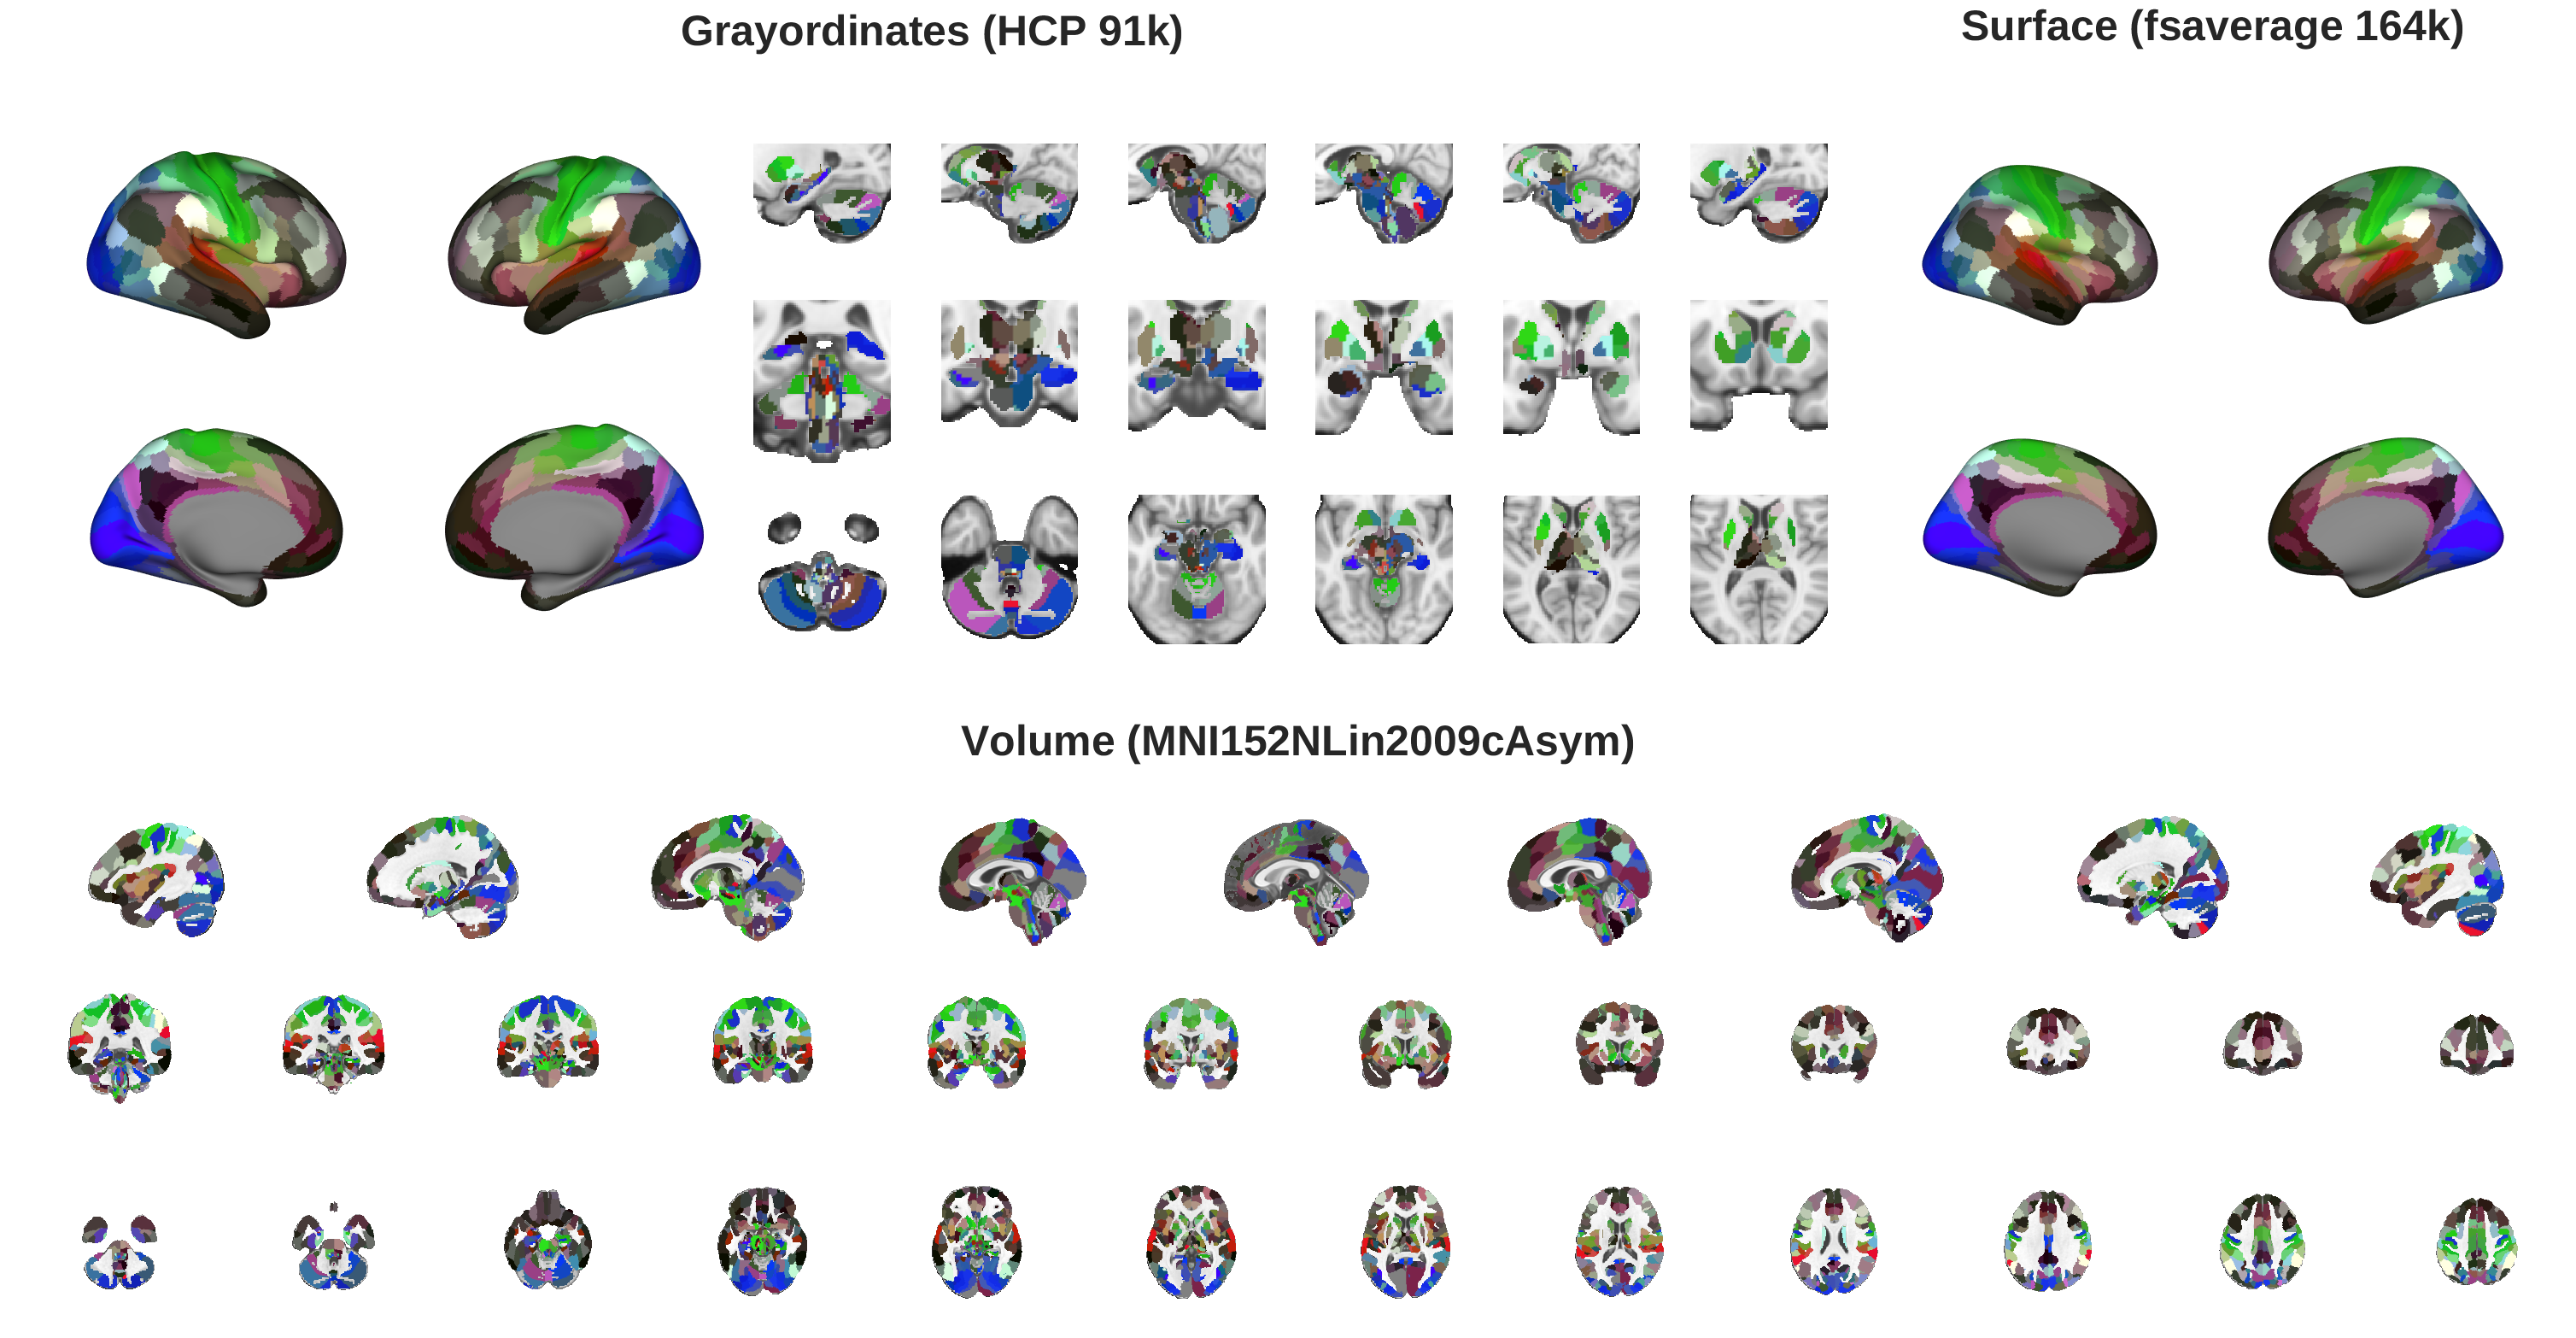
\includegraphics[width=\textwidth]{images/overview_figure.png}
\caption{{\bf CANLab2024, at its most granular, illustrated in multiple spaces.} 601 parcels are shown, 358 cortical, 243 subcortical. Grayordinates are shown on the S1200 HCP 91k inflated surface or a MNI152NLin6Asym template underlay. Surface labels are shown on the fsaverage 164k inflated surface. Meanwhile, volumetric plots use a MNI152NLin2009cAsym underlay. The tight correspondence between labels, surfaces and underlays qualitatively illustrates the precision and versatility of our labels. Colors adapted from \shortcite{Glasser2016}.}
\label{overview-figure}
\end{figure*}

An overview of the CANLab2024 atlas is presented in figure \ref{overview-figure}.

\subsection{Overview of parcellations}
Each structure is subdivided into multiple nested levels of parcels. Here we will present each gross structure and nested parcellations thereof. There are four levels of nesting (Figure \ref{granularities-overview-figure}). Level 1 is optimized for signal attribution and reverse inference, but many structures are likely too small and inconsistently localized for robust use in may applications. For instance, the typical T2* EPI imaging sequences sample the brain with 3mm isotropic voxels, and the point spread function of the BOLD signal at 3T has a full width half maximum of 3mm [citation needed], corresponding to an effective spatial resolution of 27mm$^3$, but in a forced choice parcellation scheme 21 of our finest regions have volumes smaller than this. These regions may be useful for reverse inference, since their probability maps extend over a larger region of space, but in most of that space neighboring structures are more probable and would be selected instead by deterministic parcellation schemes. Level 2 provides an alternative, designed for tractography, deterministic parcellation and region of interest analysis. Level 3 offers a coarser alternative to level 2 possibly better suited to legacy data and registration techniques or computationally demanding applications. Level 4 provides a natural grouping of finer levels of granularity (e.g. Caudate, Putamen, Hippocampal formation, cerebellar cortex, etc.) to facilitate targeted analysis of large scale structures. For cortex and cerebellum, no extremely small parcels exist, and therefore levels 1 and 2 are redundant. Parcellations at each scale for each large scale structure are detailed below.

\begin{figure*}[t]
\centering
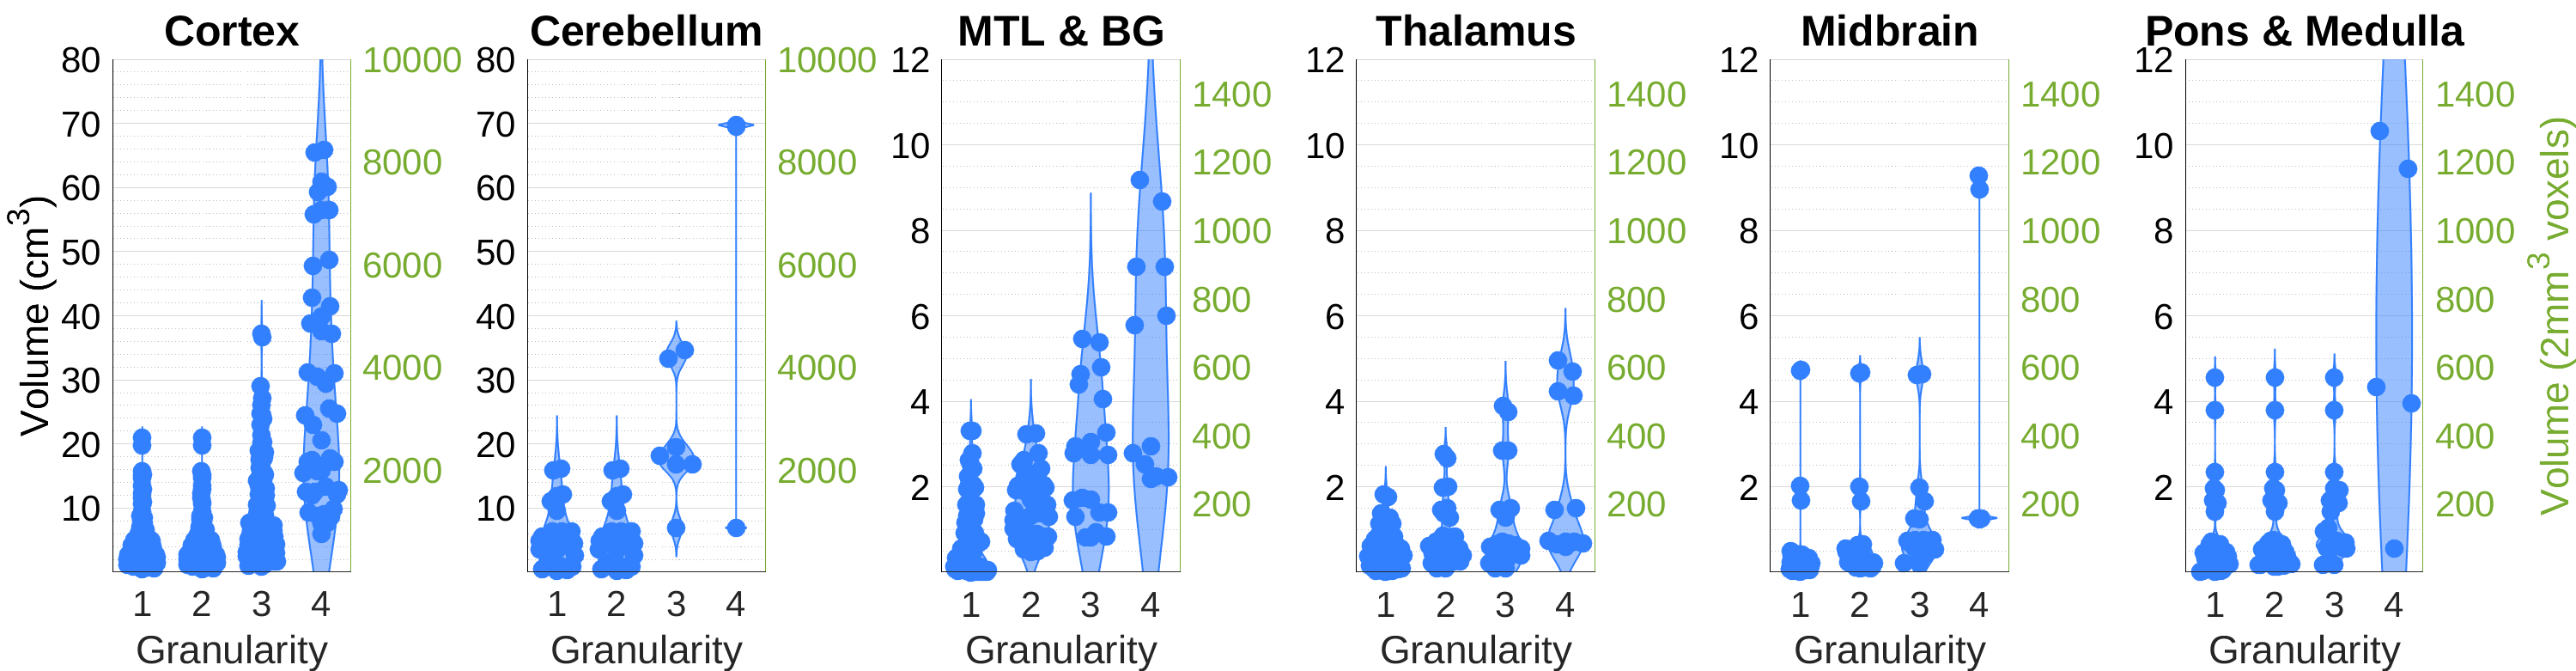
\includegraphics[width=\linewidth]{images/parcel_sizes.png}
\caption{
{\bf
Four nested parcellation are available which vary in granularity from fine to coarse to help balance between the demands of different use cases.} Some regions are difficult to localize at the resolution of popular registration templates (2mm$^3$ isotropic, right axes). Fine scale regions are merged with functional or structurally related neighbors to produce coarser granularities that may be more practical in some applicaitons. MLT: medial temporal lobe; BG: basal ganglia.
}
\label{granularities-overview-figure}
\end{figure*}

\subsubsection{Cortex} 
Probabilistic labels (Figure \ref{}); Granularities (Figure \ref{cortex-granularities-figure})
[compare with Huang et al. 2022 Brain Structure and Function and Horn et al 2016]


\begin{figure}[t]
\centering
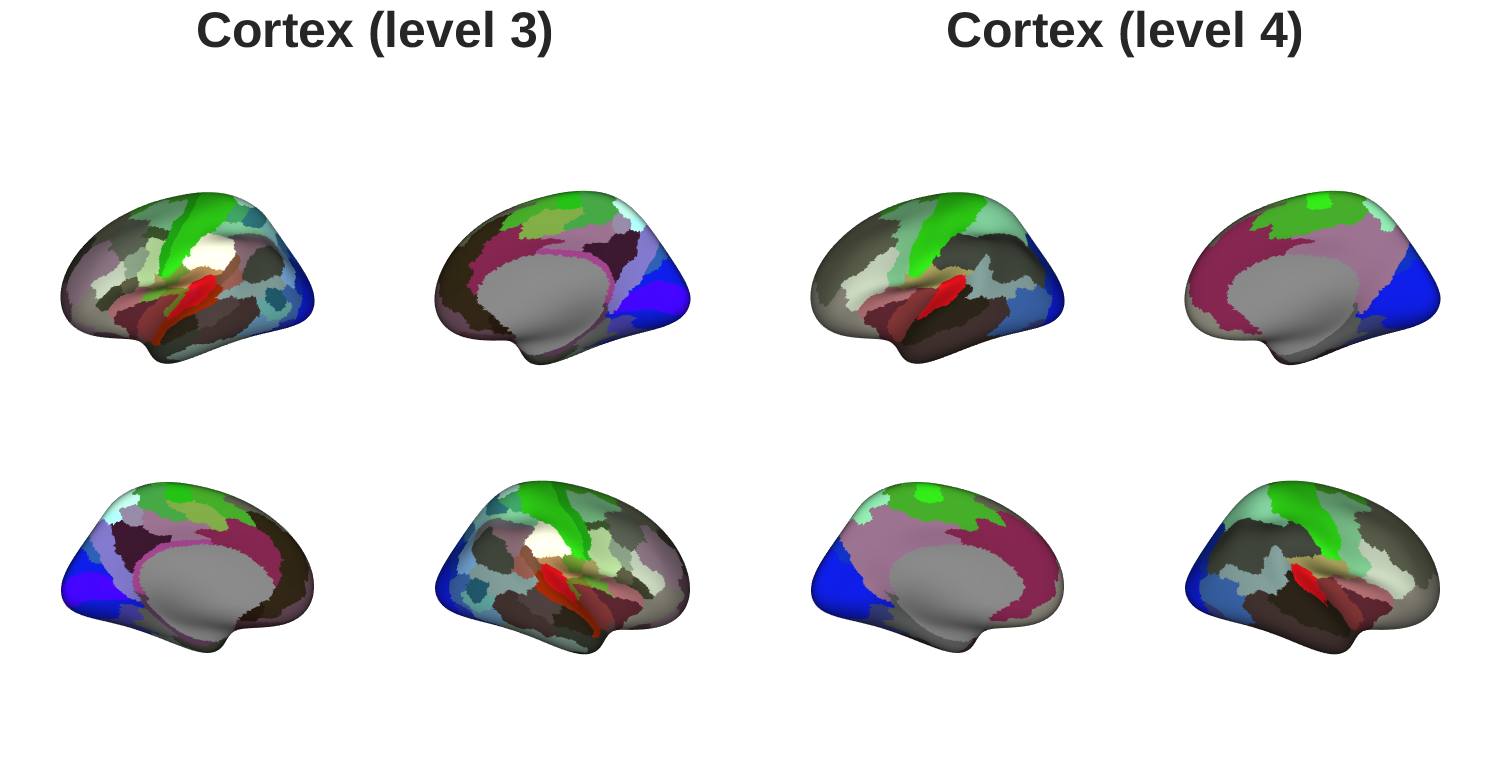
\includegraphics[width=\linewidth]{images/cortex_label_granularities.png}
\caption{
{\bf
CANLab2024 cortical parcels: coarser subdivisions.} 
The finest granularity of cortical parcels (level 1) was shown in Figure \ref{overview-figure}, but two coarser parcellations are also available (level 3 and level 4). Levels 2 is generally a downsampled version of level 1 that is more suitable for practical use as a priori ROIs, but in the case of the cortical parcels all regions were already large enough for such use, so no additional downsampling was used at level 2, and it is redundant with level 1.}
\label{cortex-granularities-figure}
\end{figure}

\subsubsection{Thalamus}
[this requires some attention to the habenula and it's relationship with neighboring structures. Commentary is also needed in differences between 1mm and 2mm versions of the atlas, in particular, at 2mm there are no midline structures (where do they go? Are they subsumed by rostral intralaminar [rIL] regoins?)]

Figure \ref{thalamus-granularities-figure}

\begin{figure}[t]
\centering
\begin{minipage}{\linewidth}
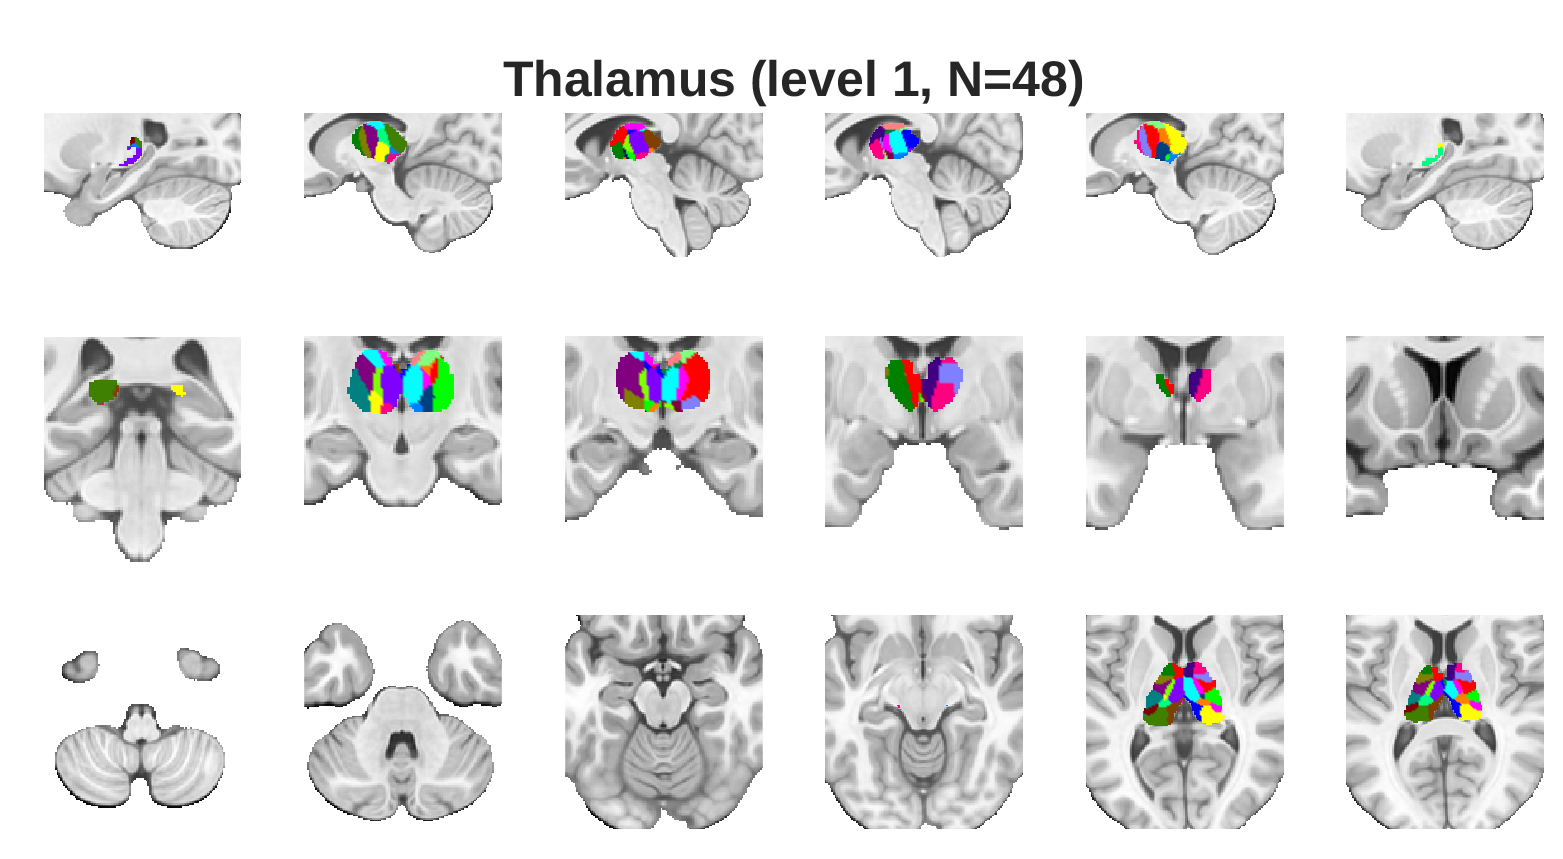
\includegraphics[width=\linewidth]{images/thal_fine.png}
\end{minipage}
\begin{minipage}{\linewidth}
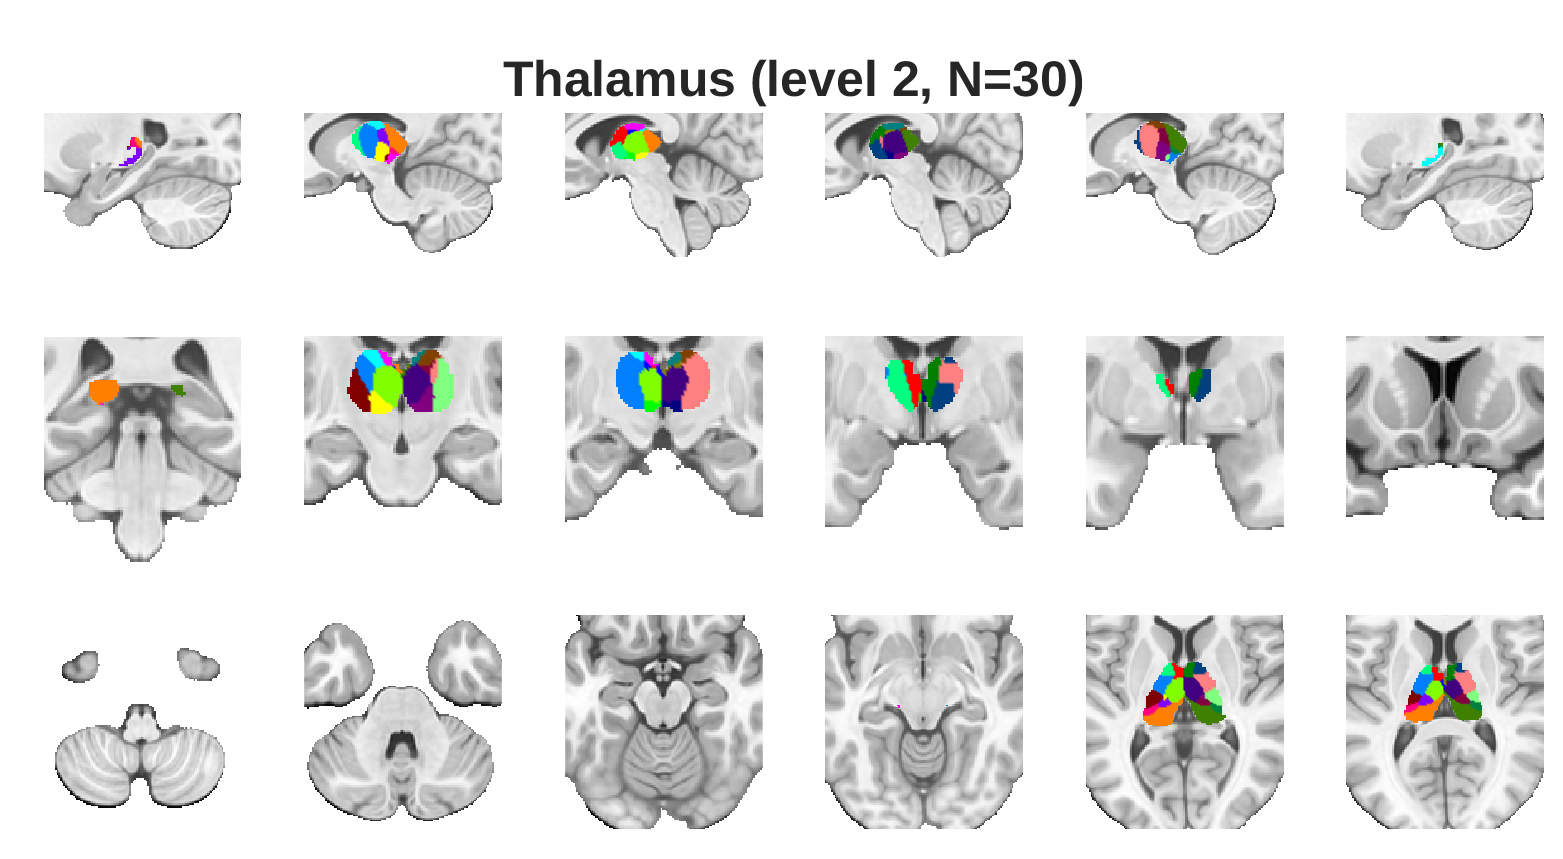
\includegraphics[width=\linewidth]{images/thal_coarse.png}
\end{minipage}
\begin{minipage}{\linewidth}
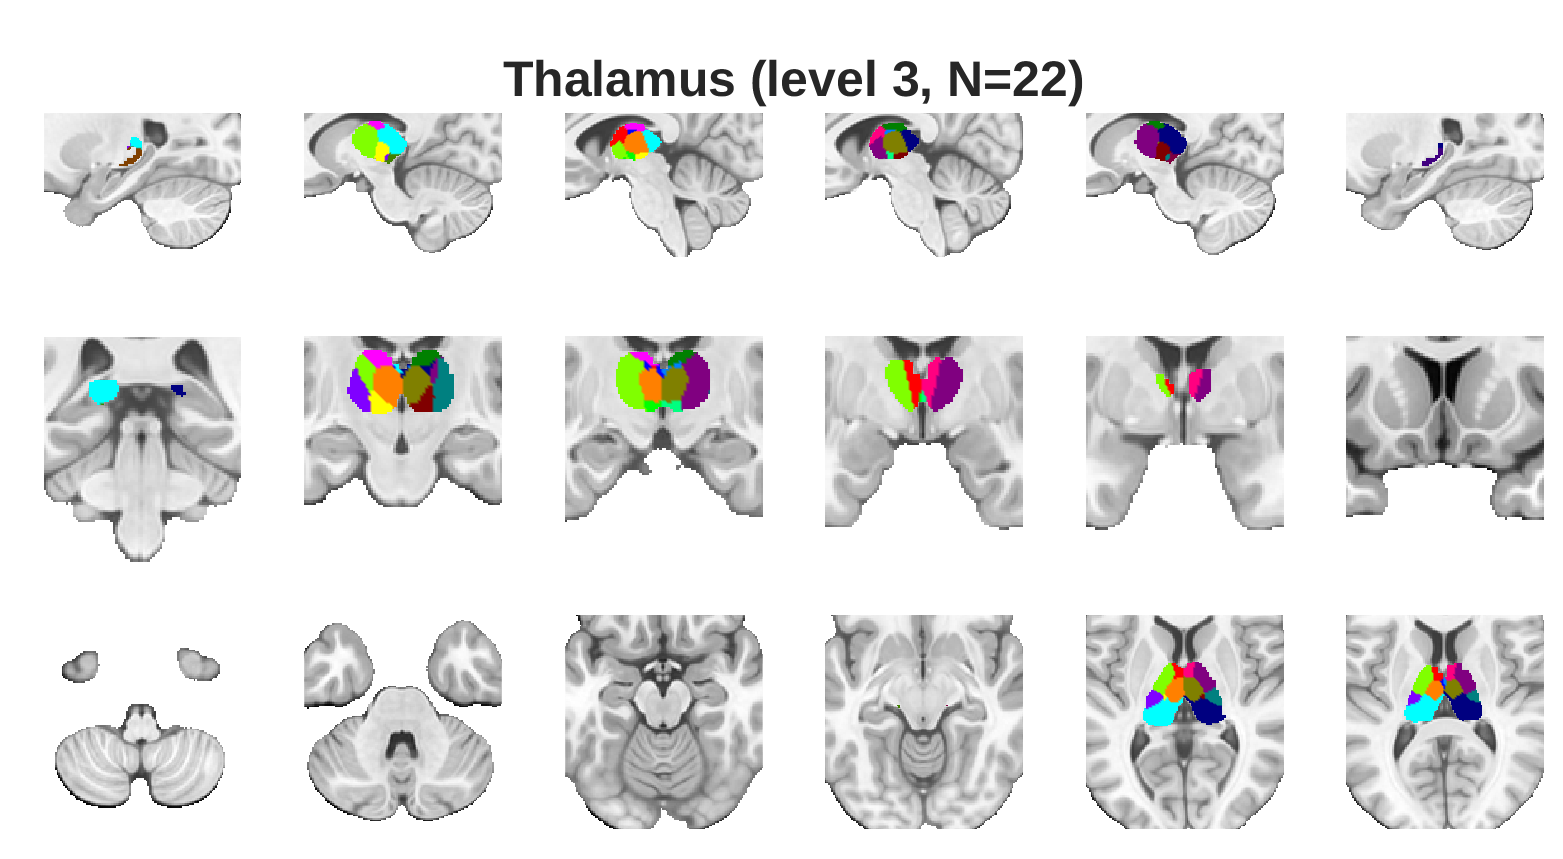
\includegraphics[width=\linewidth]{images/thal_coarser.png}
\end{minipage}
\begin{minipage}{\linewidth}
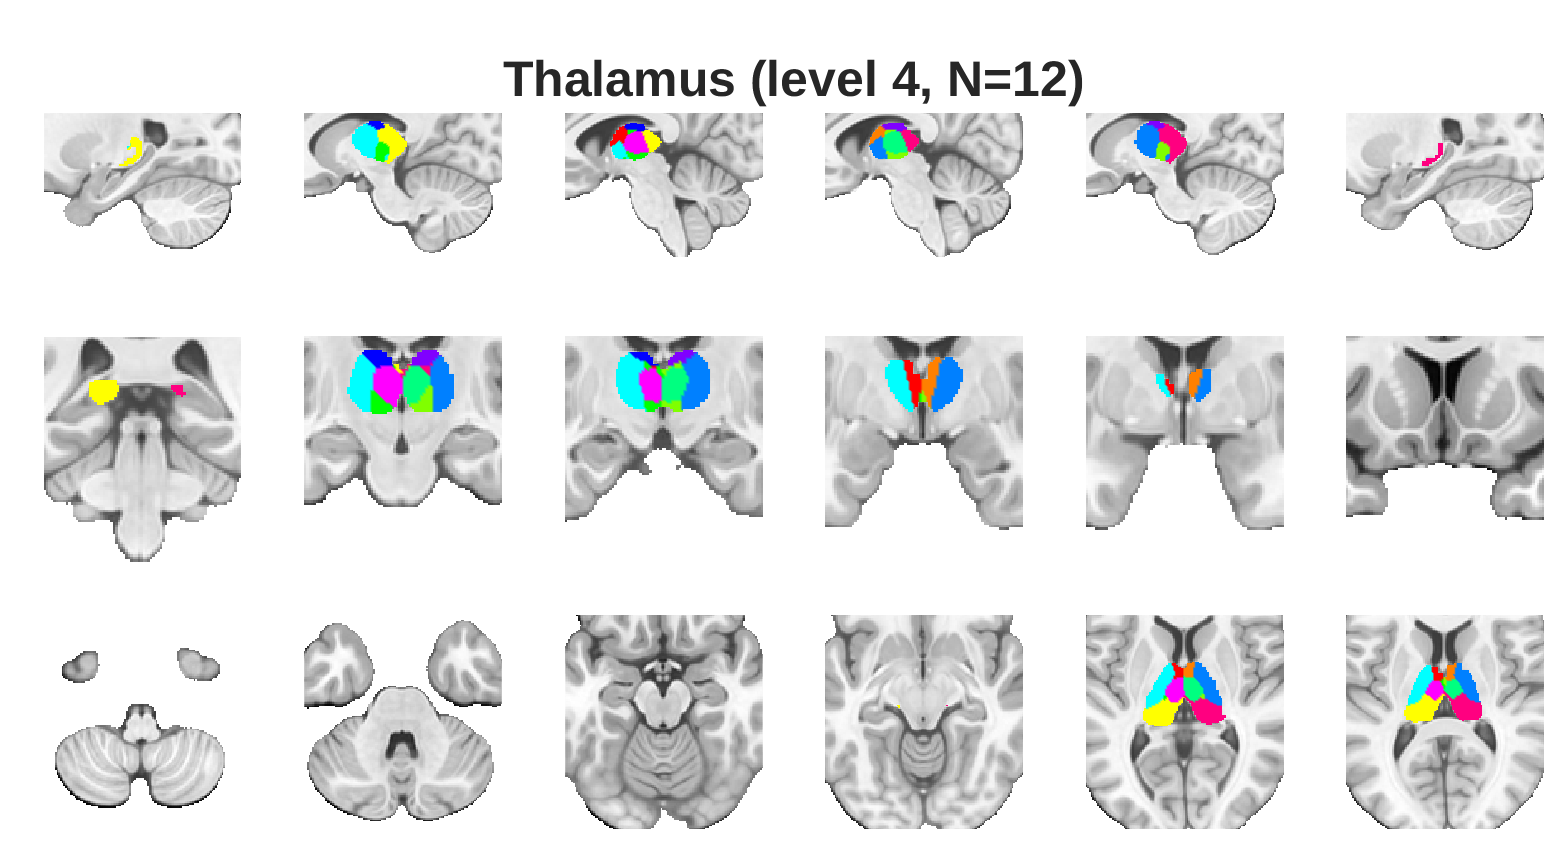
\includegraphics[width=\linewidth]{images/thal_coarsest.png}
\end{minipage}
\caption{
{\bf
CANLab2024 thalamic parcels} 
}
\label{thalamus-granularities-figure}
\end{figure}

\subsubsection{Basal Ganglia}

\begin{figure}[t]
\centering
\begin{minipage}{\linewidth}
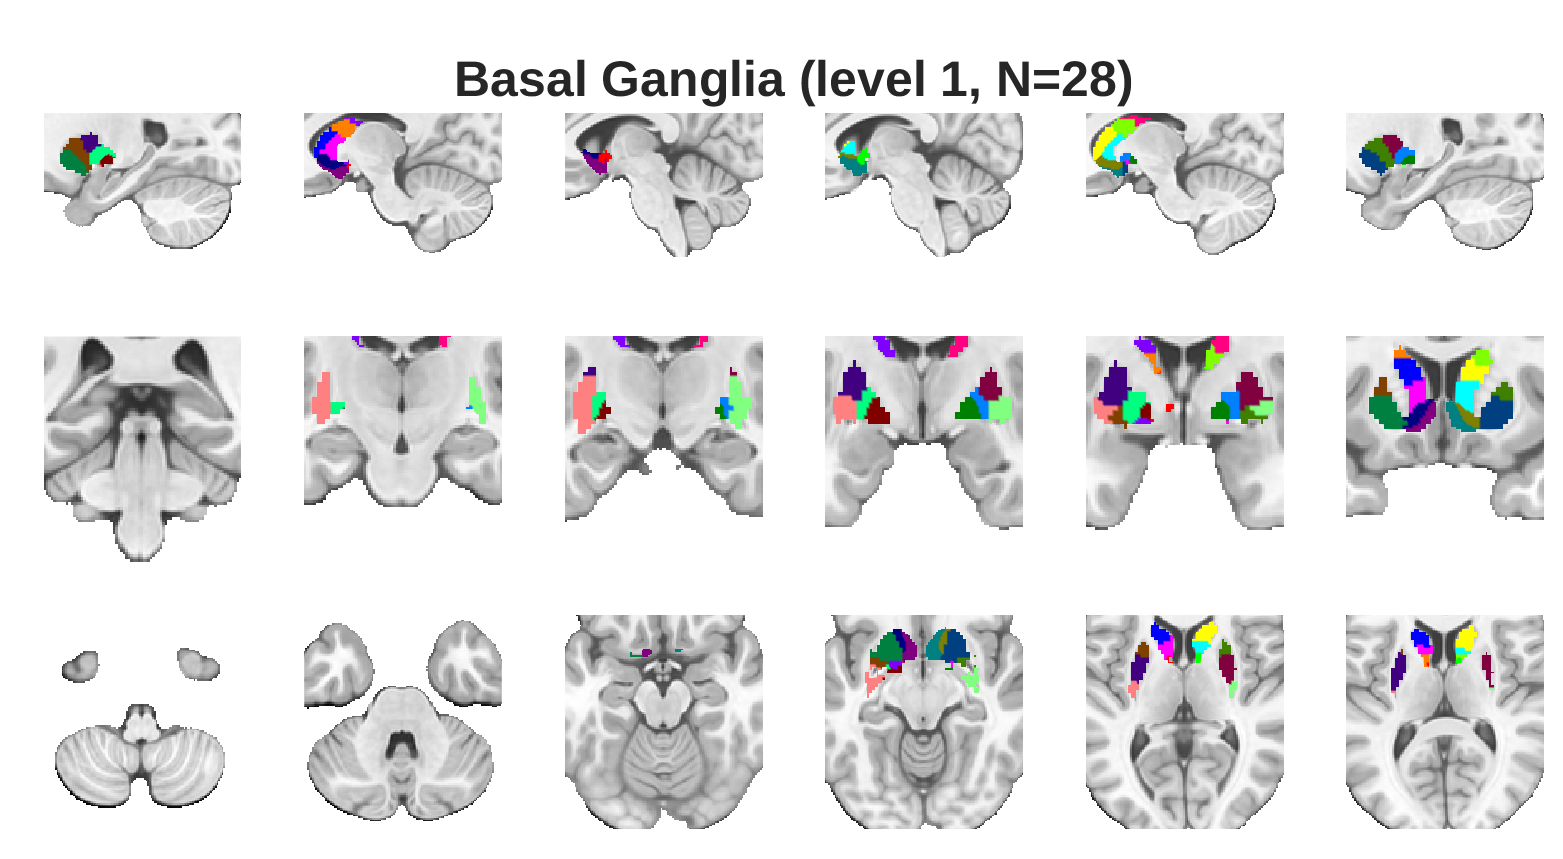
\includegraphics[width=\linewidth]{images/bg_fine.png}
\end{minipage}
\begin{minipage}{\linewidth}
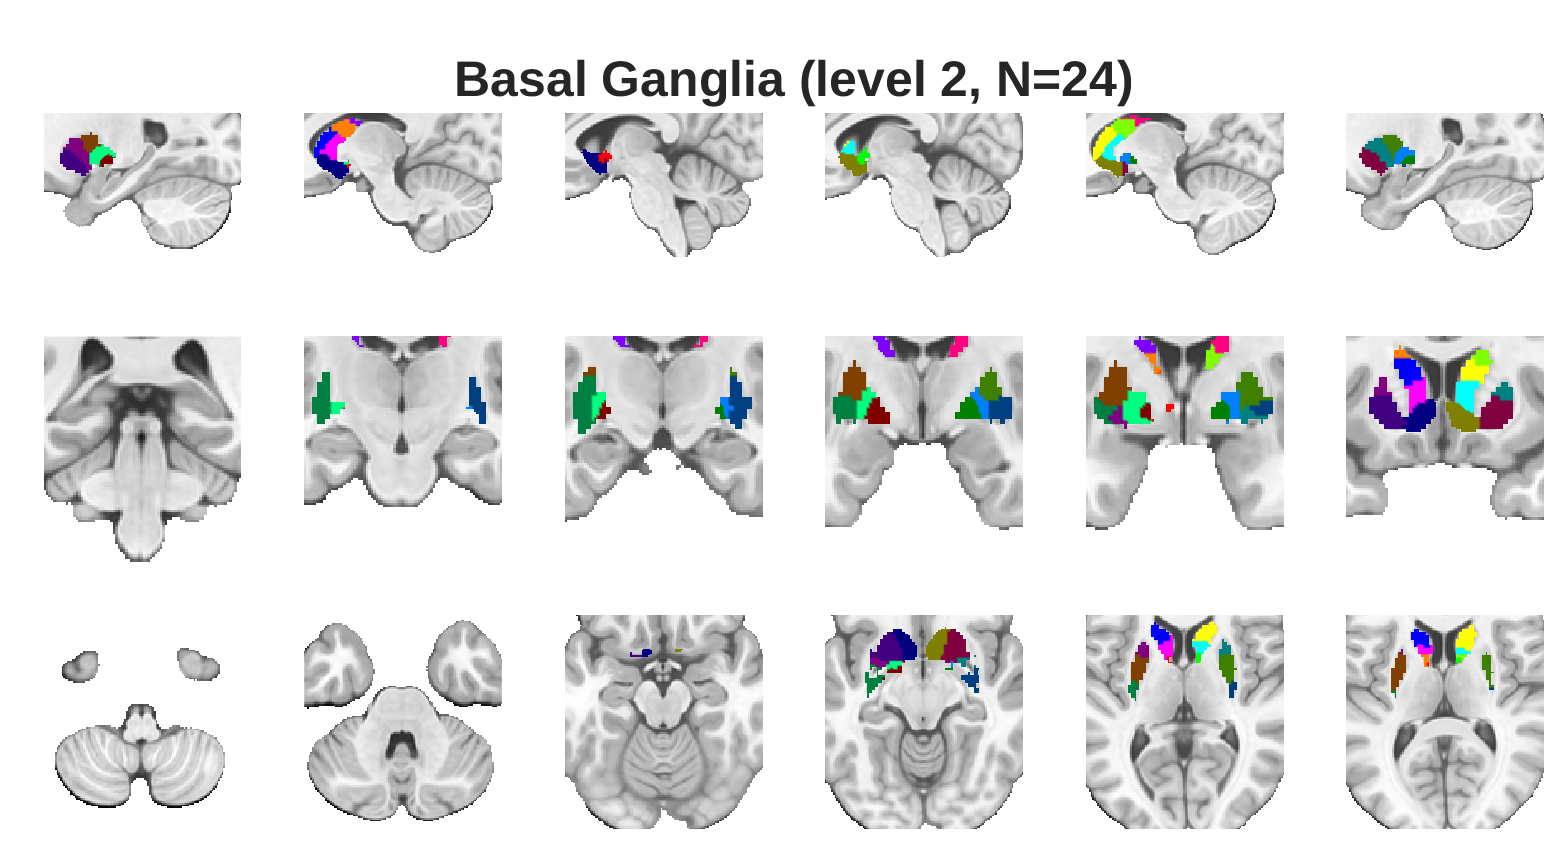
\includegraphics[width=\linewidth]{images/bg_coarse.png}
\end{minipage}
\begin{minipage}{\linewidth}
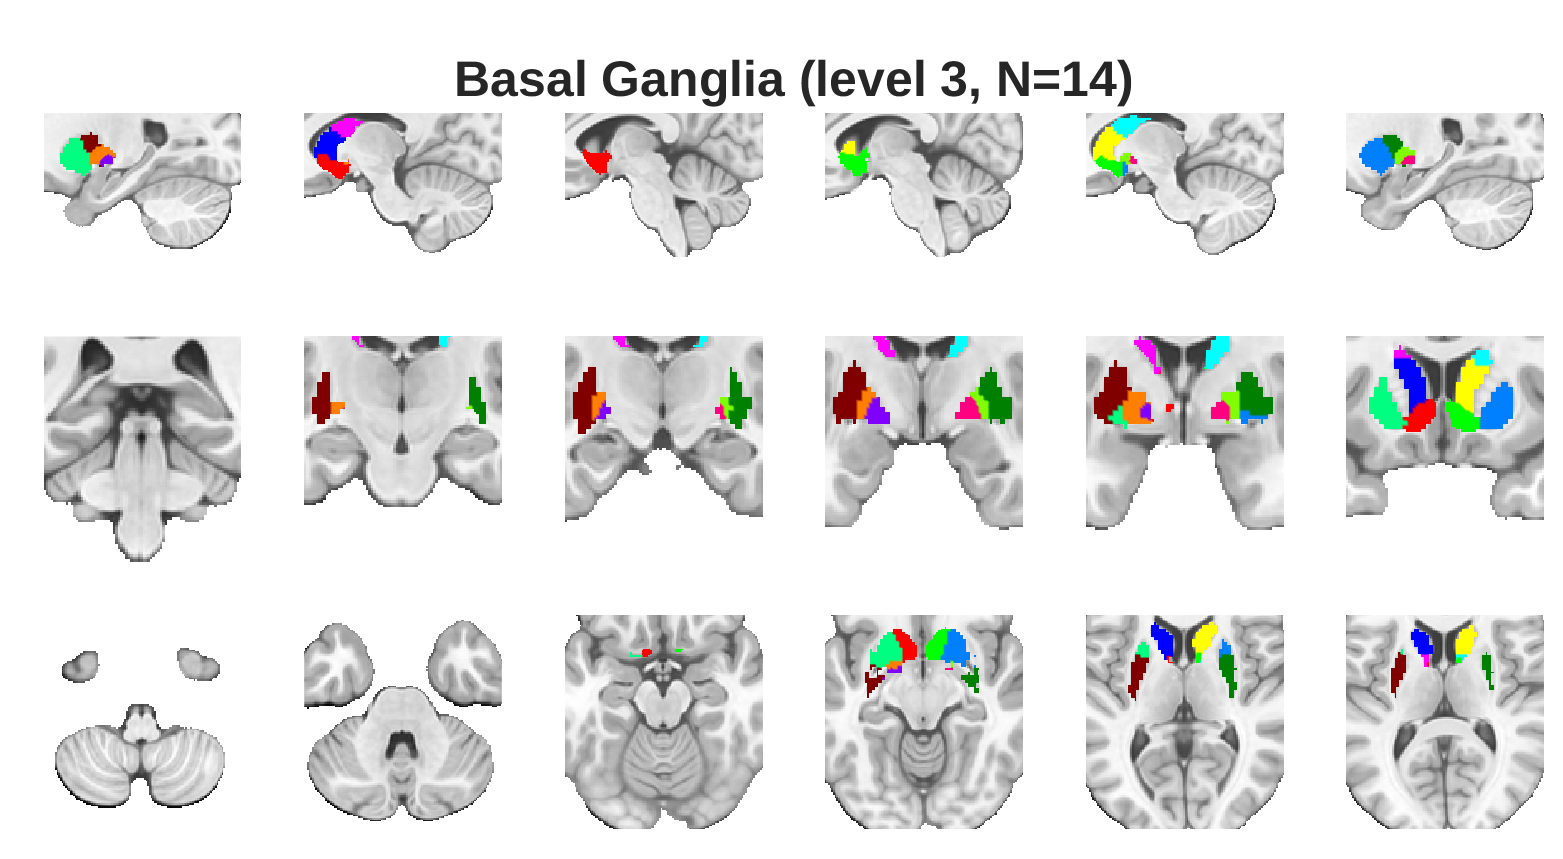
\includegraphics[width=\linewidth]{images/bg_coarser.png}
\end{minipage}
\begin{minipage}{\linewidth}
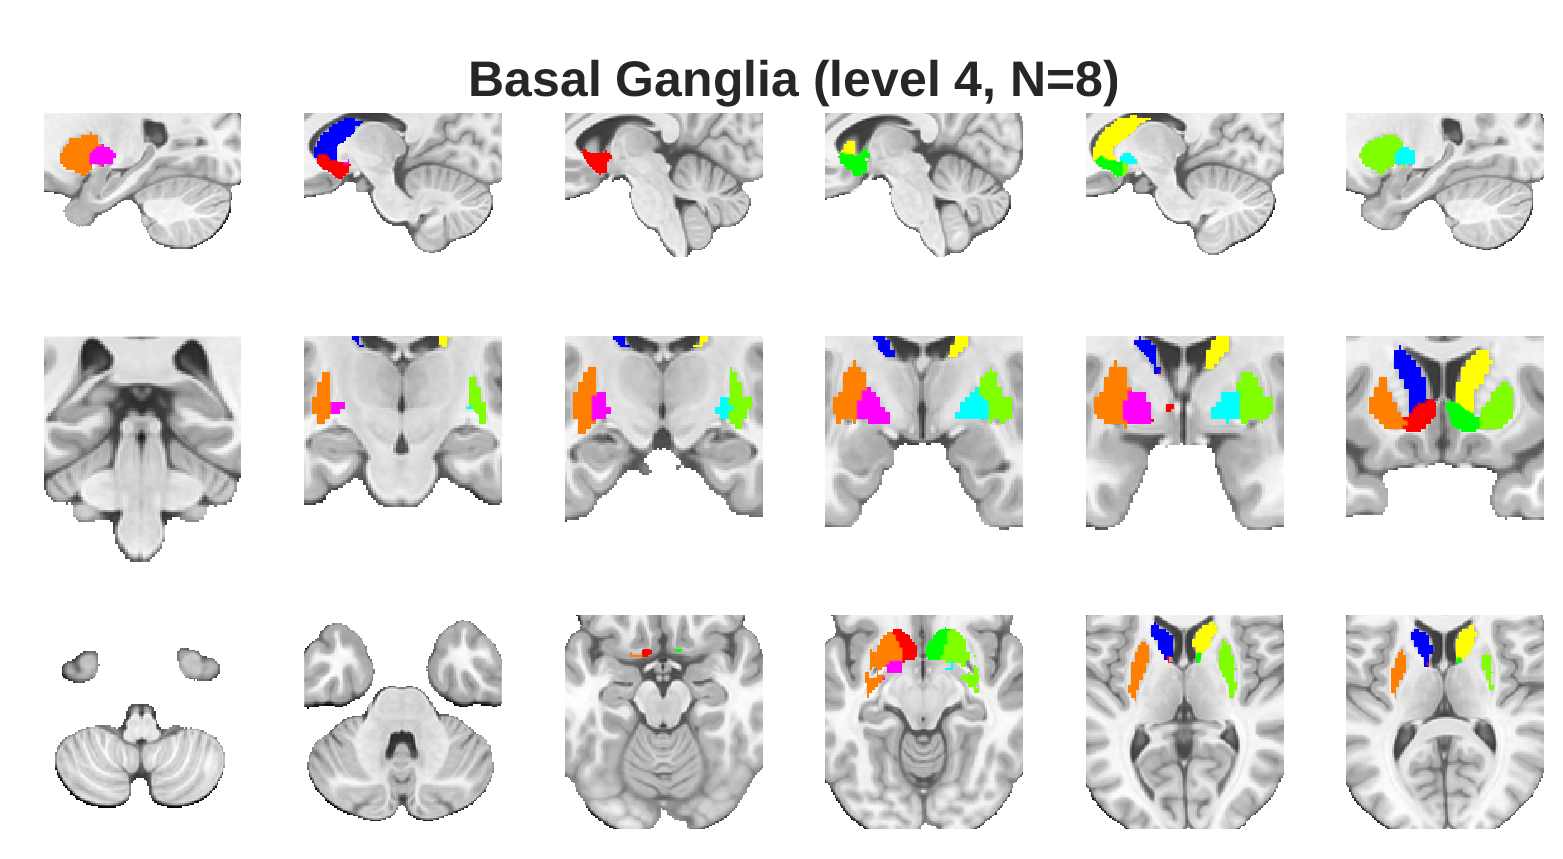
\includegraphics[width=\linewidth]{images/bg_coarsest.png}
\end{minipage}
\caption{
{\bf
CANLab2024 basal ganglia parcels} 
}
\label{bg-granularities-figure}
\end{figure}

The basal ganglia in CANLab2024 are one of two categories of structures where labels differ in volumetric and grayordinate atlases. The basal ganglia are constituted by parcels from Tian, Cartmell and CIT atlases. Although Tian is derived from the same data used to define the grayordinate space (HCP), and therefore abides by the grayordinate boundaries perfectly, CIT and Cartmell do not. To better accommodate ventral striatal regions derived from these atlases the volumetric parcels were allowed to exceed the CIFTI boundaries slightly, which is most visible when comparing the left (red) and right (green) ventral striatal parcels in Figure \ref{bg-vs-cifti-figure} with the grayordinate parcel boundaries (black outlines). This introduces slight differences between volumetric and CIFTI versions of CANLab2024, since these areas outside of the grayordinate boundaries and are therefore absent in the latter. 

Notably, the divisions between accumbens/putamen and accumbens/caudate are also not identical to the grayordinate structures, which limits the utility of grayordinate structural labels when using this atlas. For instance, using connectome workbench to extract the ``ACCUMBENS\_LEFT" structure will select only a subset of the CANLab2024 accumbens, while trying to extract ``CAUDATE\_LEFT" will result in a mixture of caudate and ventral striatum parcels. This inconsistency across atlases is consistent with the absence of clear criteria for delineating the transitions between these regions \shortcite{Haber2010, Tian2020}, but we believe that functional \shortcite{Tian2020} and tractography based criteria \shortcite{Cartmell2019} should take precedence over the gray matter contrast based criteria according to which the grayordinate labels were defined [citation needed].

Finally, Figure \ref{bg-vs-cifti-figure} illustrates the absence of the most lateral voxels of the putamen which were excluded from our parcellation due to their frequent intersection with insular vertices of surface projections. This exclusion is identical in both volumetric and grayordinate versions of the atlas.

\begin{figure*}[t!]
\centering
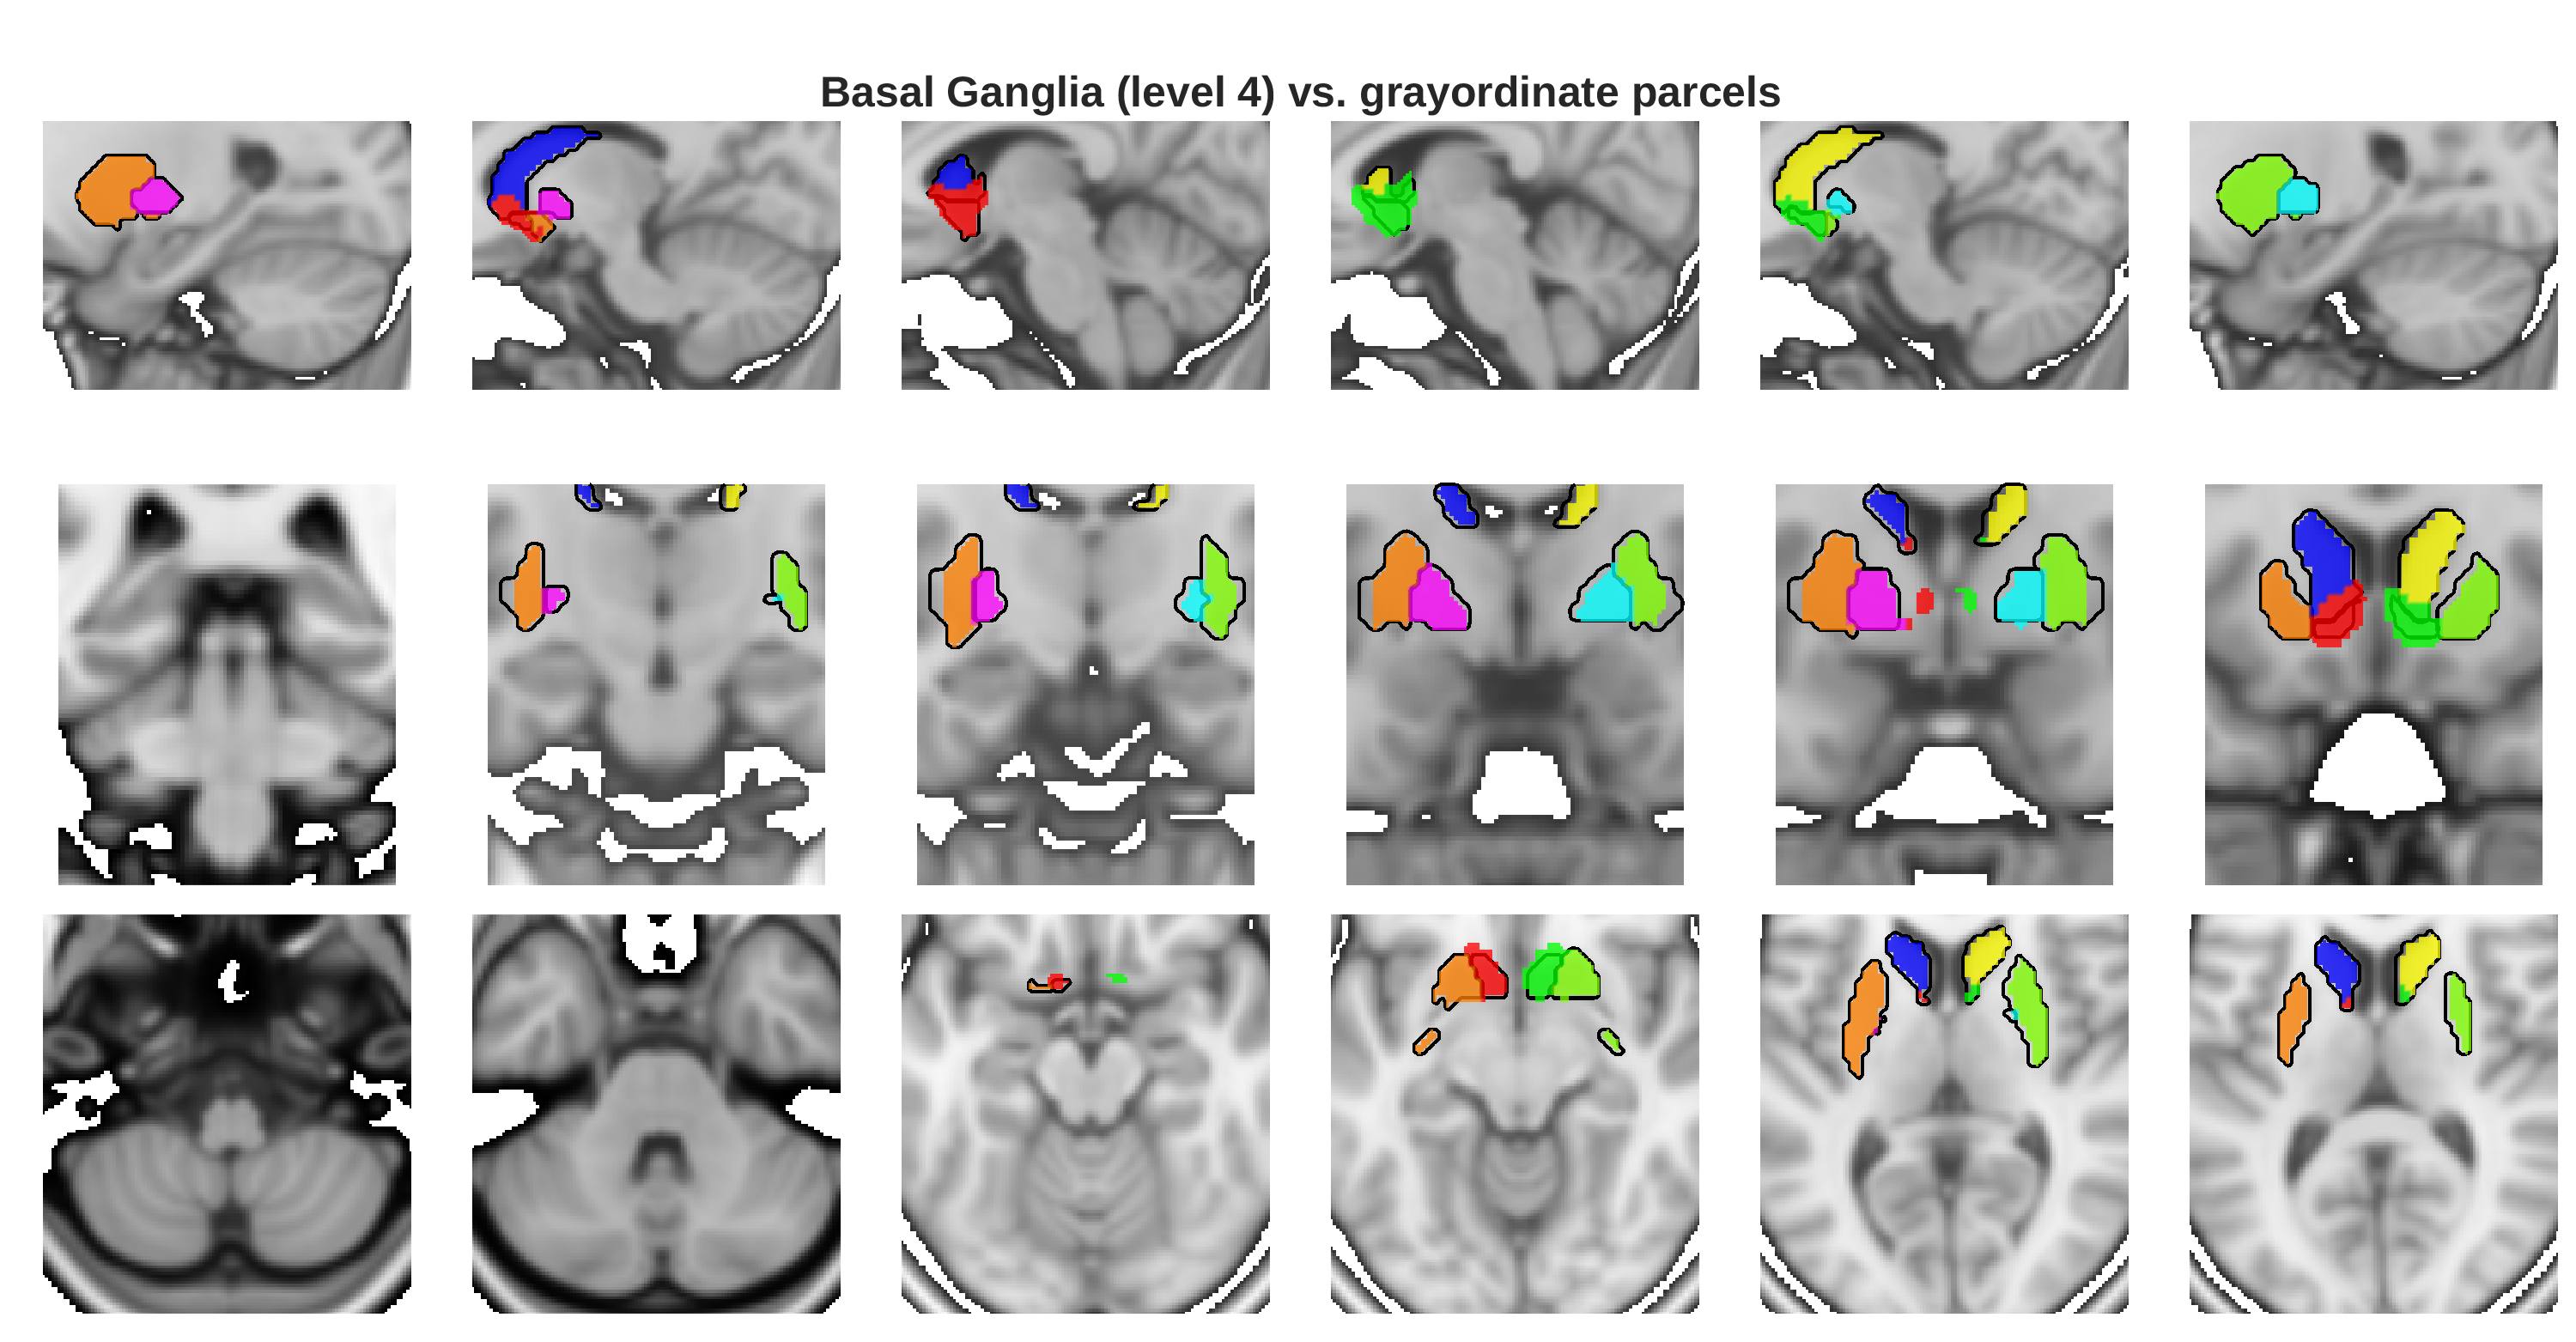
\includegraphics[width=\linewidth]{images/bg_vs_cifti.png}
\caption{
{\bf
CANLab2024 basal ganglia parcels differ from CIFTI grayordinate structural boundaries.} 
Colored outlines indicate the coarsest level of parcellation for the basal ganglia, and trace the boundaries of classic gross nuclei except for the ventral striatum which includes the nucleus accumbens as well as portions of the extended amygdala. Black lines illustrate the boundaries of corresponding structures in HCP 91k grayordinate space. CANLab2024 boundaries in the ventral striatum exceed those of the grayordinate structures, therefore grayordinate versions of the atlas will include slightly eroded ventral striatal regions relative to volumetric atlases. Meanwhile, the most lateral portions of the putamen are excluded from our atlas parcellations in all spaces despite inclusion within the grayordinate boundaries. This is to avoid redundancy with surface insular vertices with which they often overlap. Underlay: MNI152NLin6Asym T1 2mm template, used by HCP 91k grayordinates.}
\label{bg-vs-cifti-figure}
\end{figure*}

\subsubsection{Hypothalamus} 
After the basal ganglia, the hypothalamus in CANLab2024 is the only additional structures where labels differ in volumetric and grayordinate atlases. Here we include the optic nuclei anterior to the hypothalamus in our definition since these are all part of the same source atlas \shortcite{Billot2020}. These nuclei are quite small, but of particular interest since they process visual stimuli and project to thalamic areas that are highly distinct from the homeostatic function and limbic, prefrontal and brainstem projections that innervate the rest of the hypothalamus. Masking them to restrict the hypothalamus to the HCP 91k grayordinate boundaries would erode a large percentage of these optic nuclei (Figure \ref{hypothal-vs-cifti-figure}), therefore we retain these despite the incongruity it introduces between CIFTI and NIFTI versions of CANLab2024. These regions are the first to go though as we downsample our parcellation and they become subsumed by the their larger neighbors (Figure \ref{hypothal-granularities-figure}), so scope of the incongruity is limited.

\begin{figure*}[t]
\centering
\begin{minipage}{0.33\linewidth}
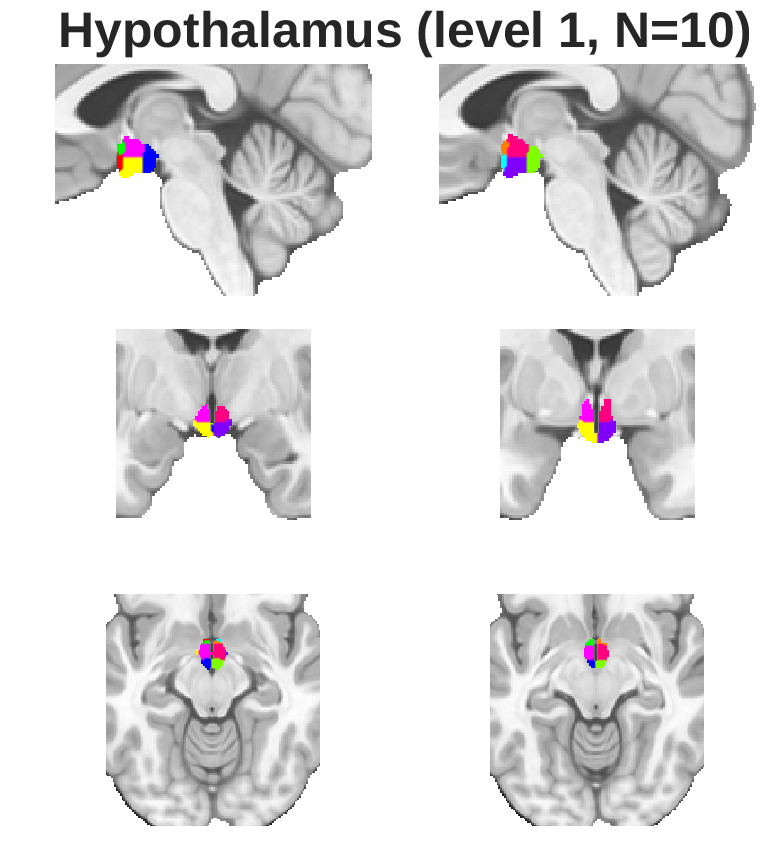
\includegraphics[width=\linewidth]{images/ht_fine.png}
\end{minipage}\hfill
\begin{minipage}{0.33\linewidth}
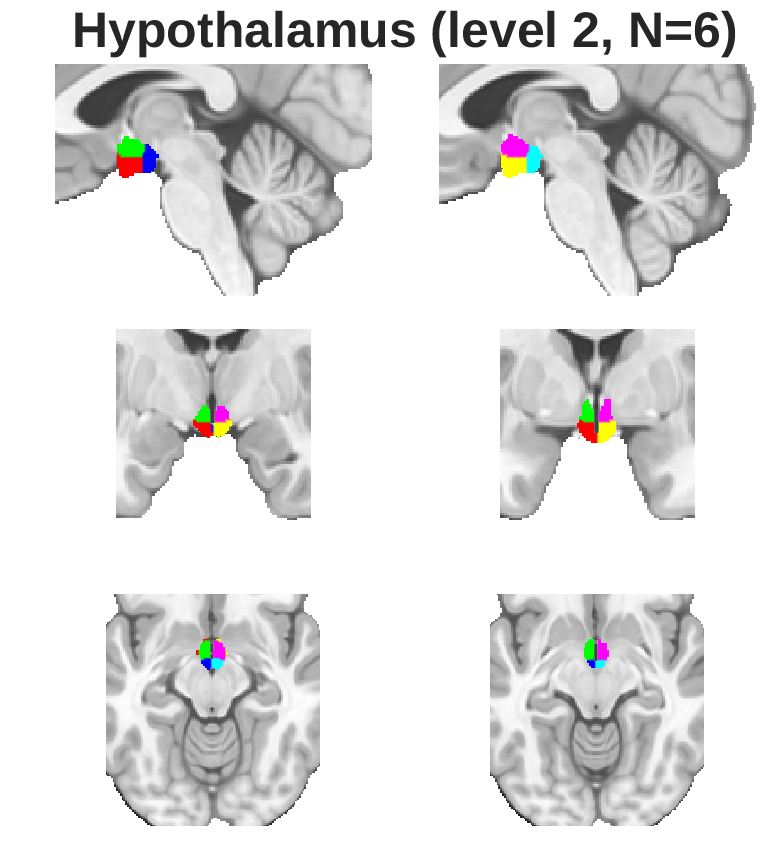
\includegraphics[width=\linewidth]{images/ht_coarse.png}
\end{minipage}\hfill
\begin{minipage}{0.33\linewidth}
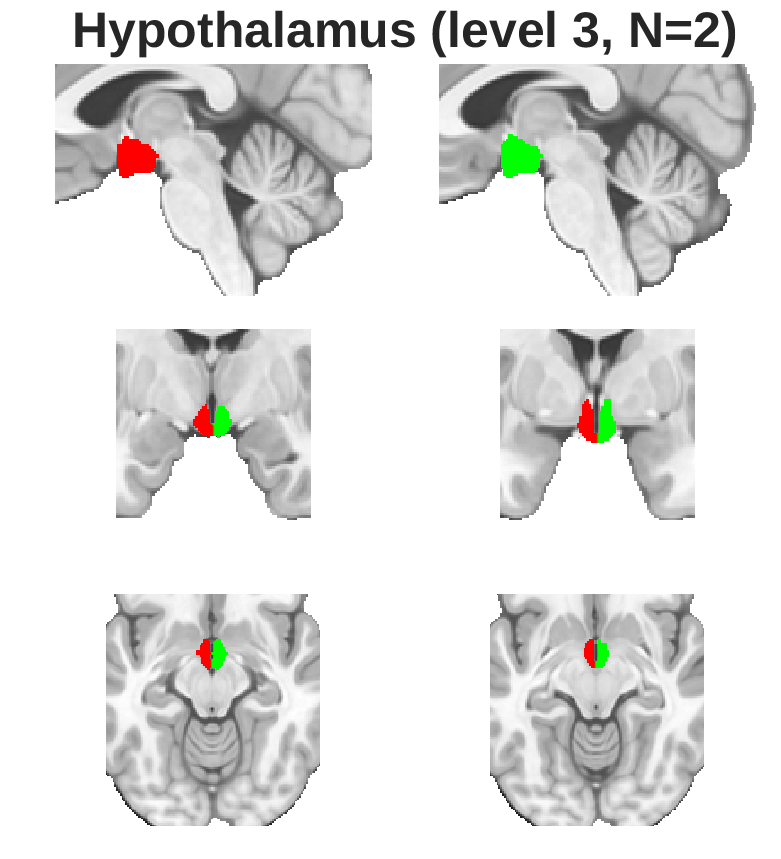
\includegraphics[width=\linewidth]{images/ht_coarser.png}
\end{minipage}\hfill
\caption{
{\bf
CANLab2024 hypothalamic parcels.} The optic nuclei are merged with anterior hypothalamic nuclei at level 2 while keeping the posterior mammillary bodies separate. All nuclei are merged at level 3. The fourth level of granularity is identical to the third (not shown).
}
\label{hypothal-granularities-figure}
\end{figure*}

\begin{figure}[t!]
\centering
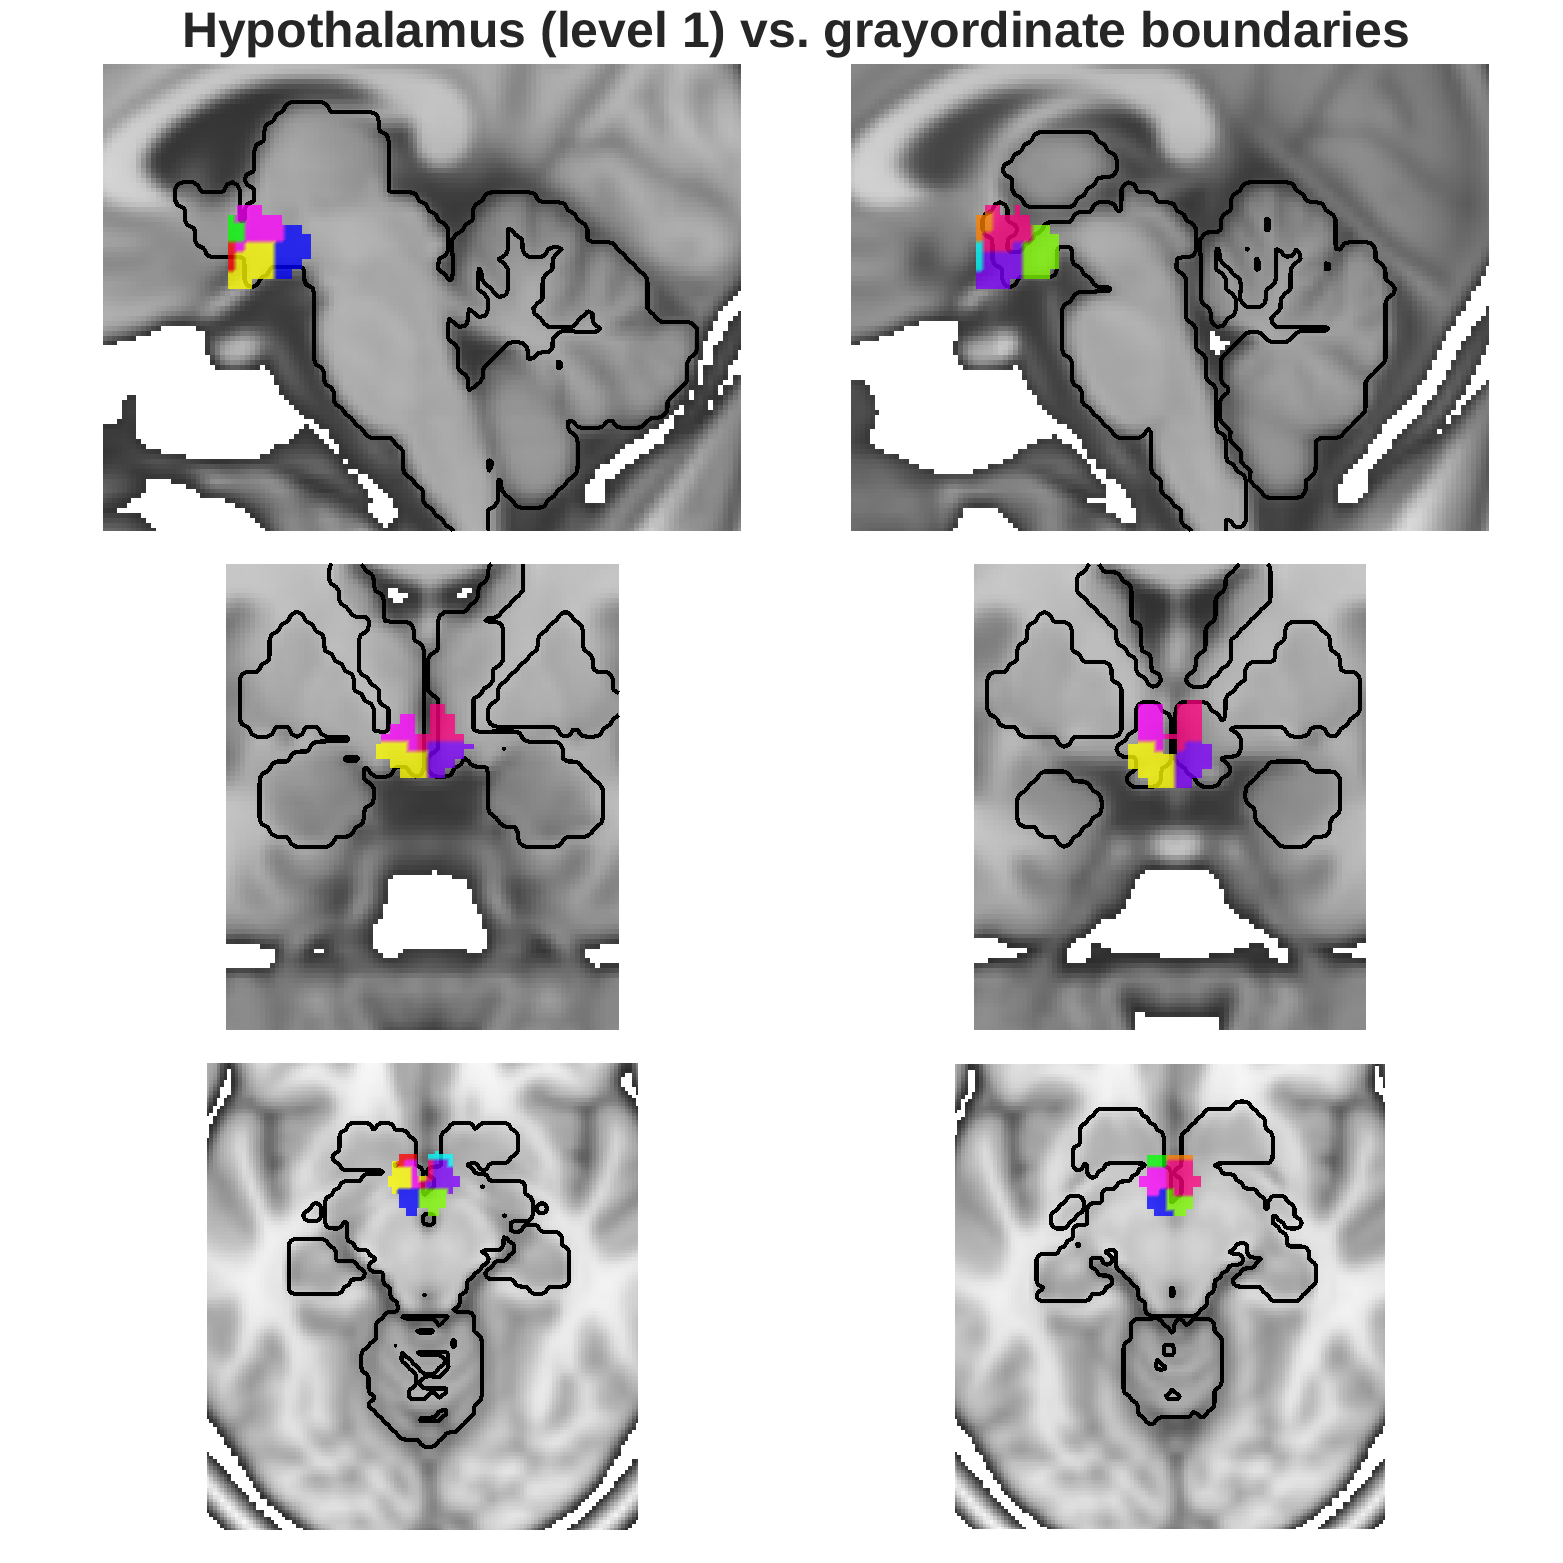
\includegraphics[width=\linewidth]{images/hypothal_vs_cifti.png}
\caption{
{\bf
CANLab2024 hypothalamus parcels exceed HCP 91k grayordinate structural boundaries.} 
Colored outlines indicate the finest level of parcellation for the hypothalamus. Black lines illustrate the boundaries of HCP 91k grayordinate space. Although the boundaries coincide well enough for most nuclei, masking the hypothalamus with grayordinate boundaries would have dramatically affected the anterior optic nuclei. Underlay: MNI152NLin6Asym T1 2mm template, used by HCP 91k grayordinates.}
\label{hypothal-vs-cifti-figure}
\end{figure}

\subsubsection{Amygdala/Hippocampus}
We describe the medial temporal lobe structures jointly because the boundaries between amygdala and hippocampus are poorly defined, so our boundaries are not guaranteed to align with those of the HCP 91k grayordinate parcels to which we project our atlas. Nevertheless, comparison of our level 4 (coarsest) labels, which subdivide the medial temporal lobe into amygdala and hippocampal formation, shows very close correspondence with the HCP 91k hippocampal and amygdala grayordinate structures.

\begin{figure}[t]
\centering
\begin{minipage}{\linewidth}
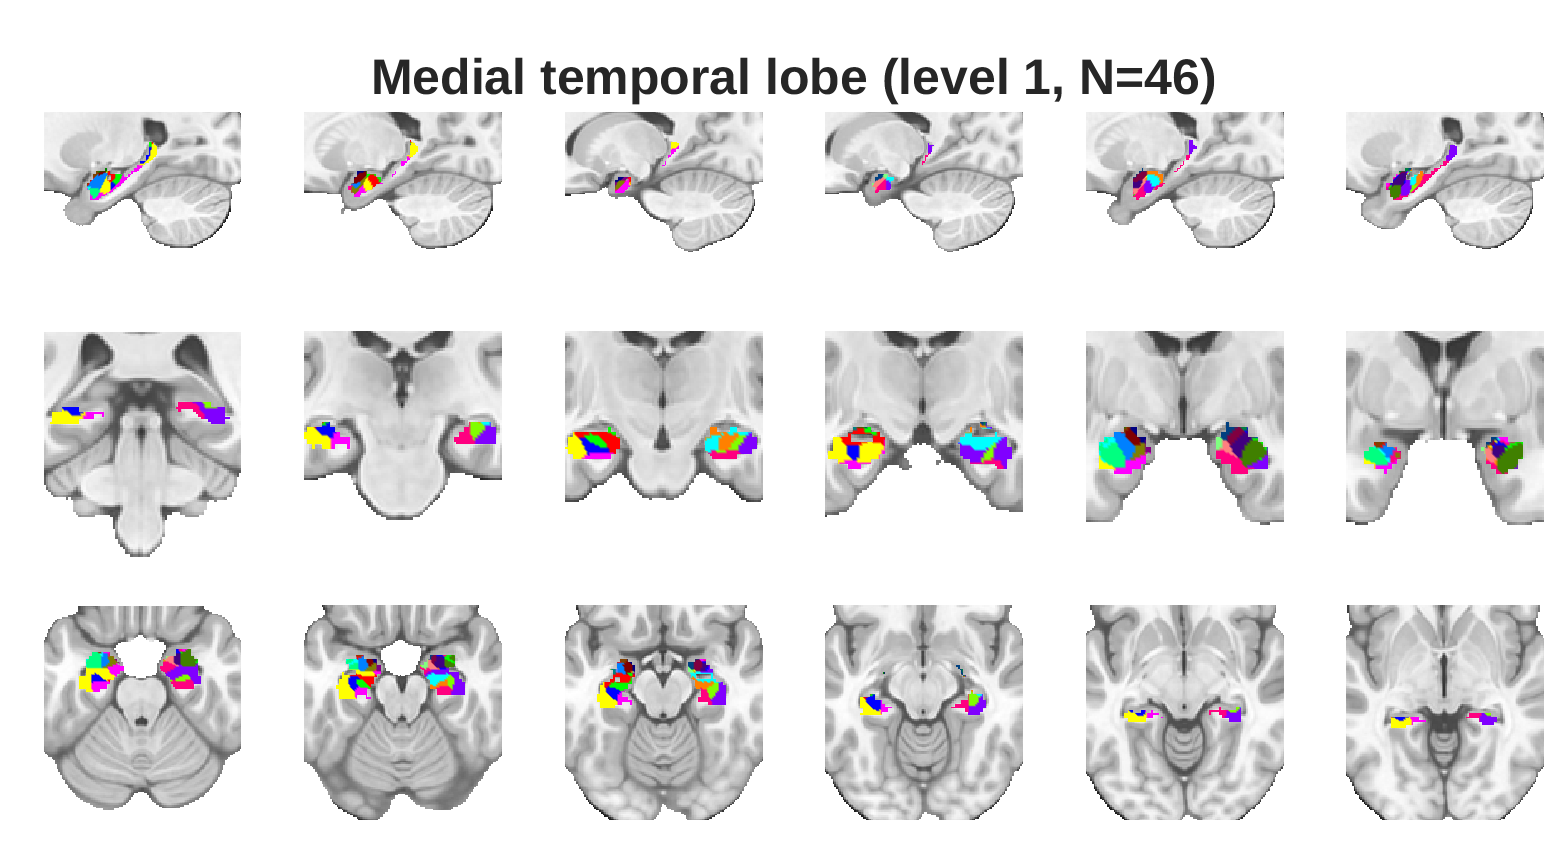
\includegraphics[width=\linewidth]{images/mtl_fine.png}
\end{minipage}
\begin{minipage}{\linewidth}
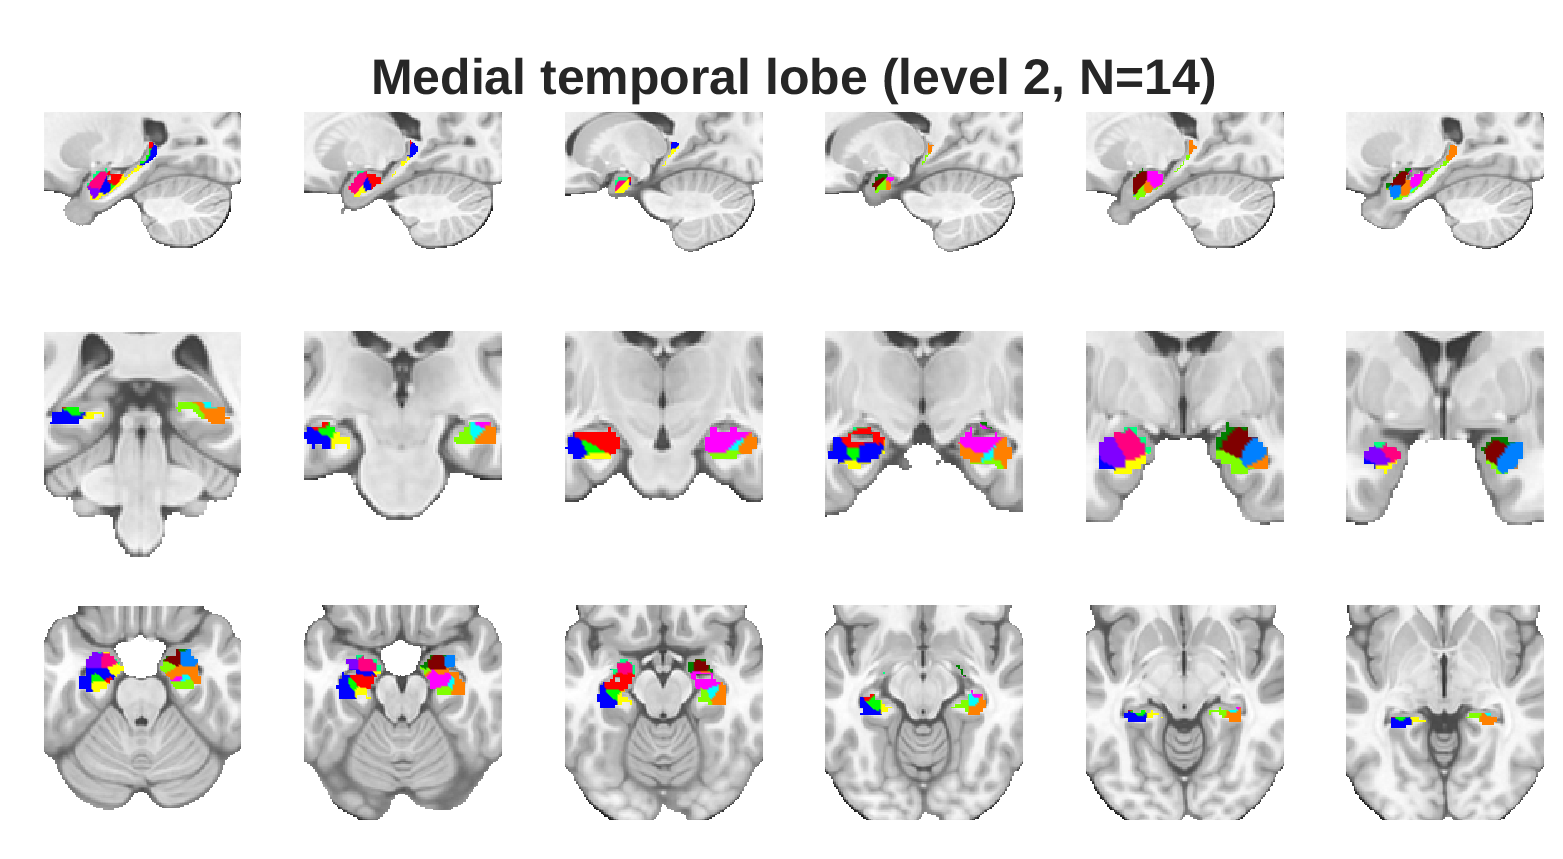
\includegraphics[width=\linewidth]{images/mtl_coarse.png}
\end{minipage}
\begin{minipage}{\linewidth}
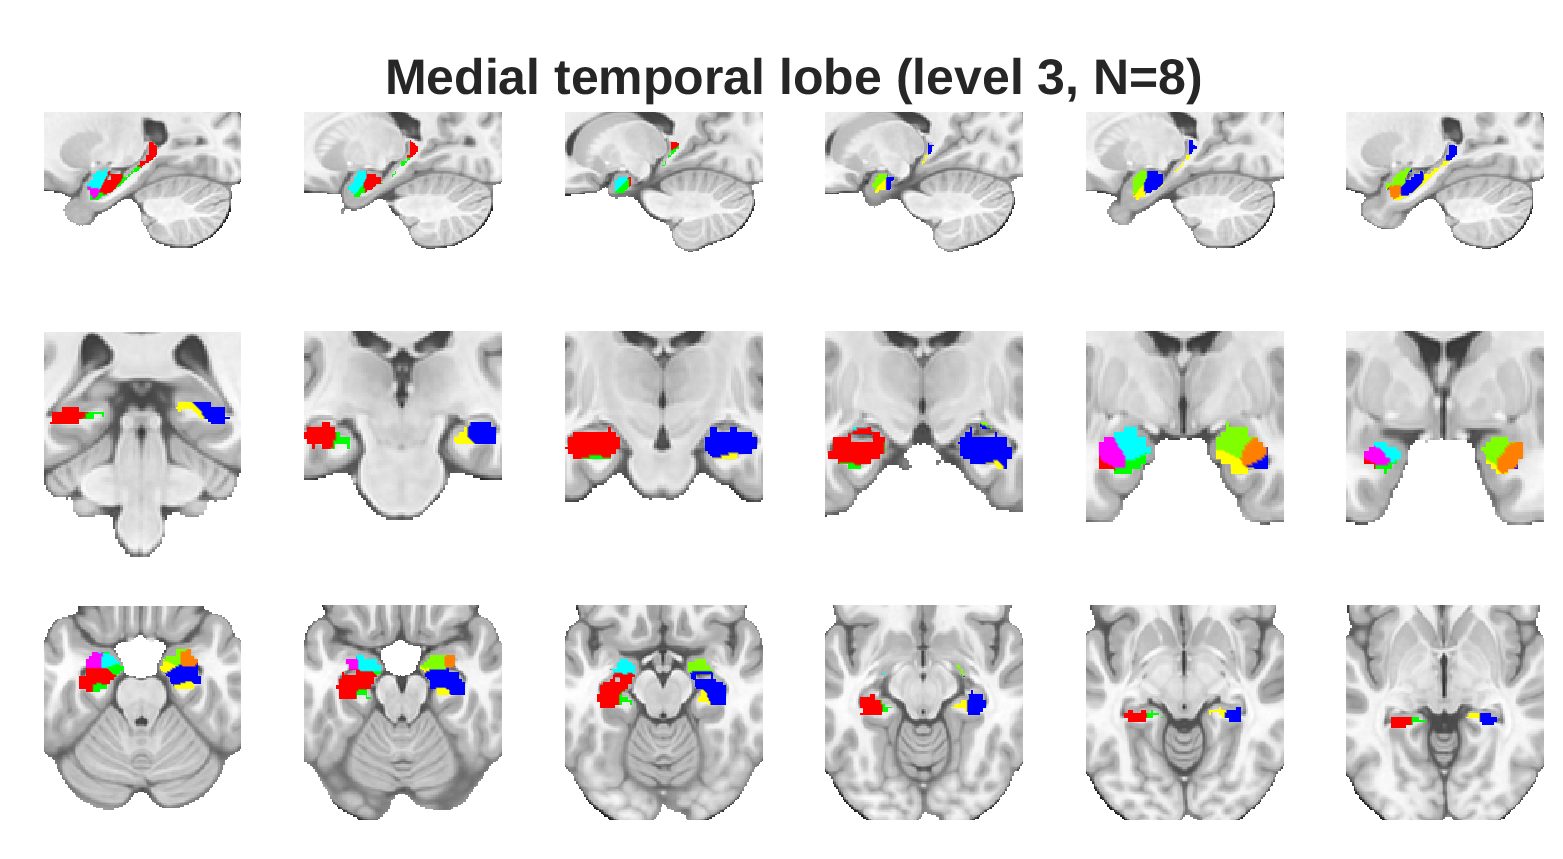
\includegraphics[width=\linewidth]{images/mtl_coarser.png}
\end{minipage}
\begin{minipage}{\linewidth}
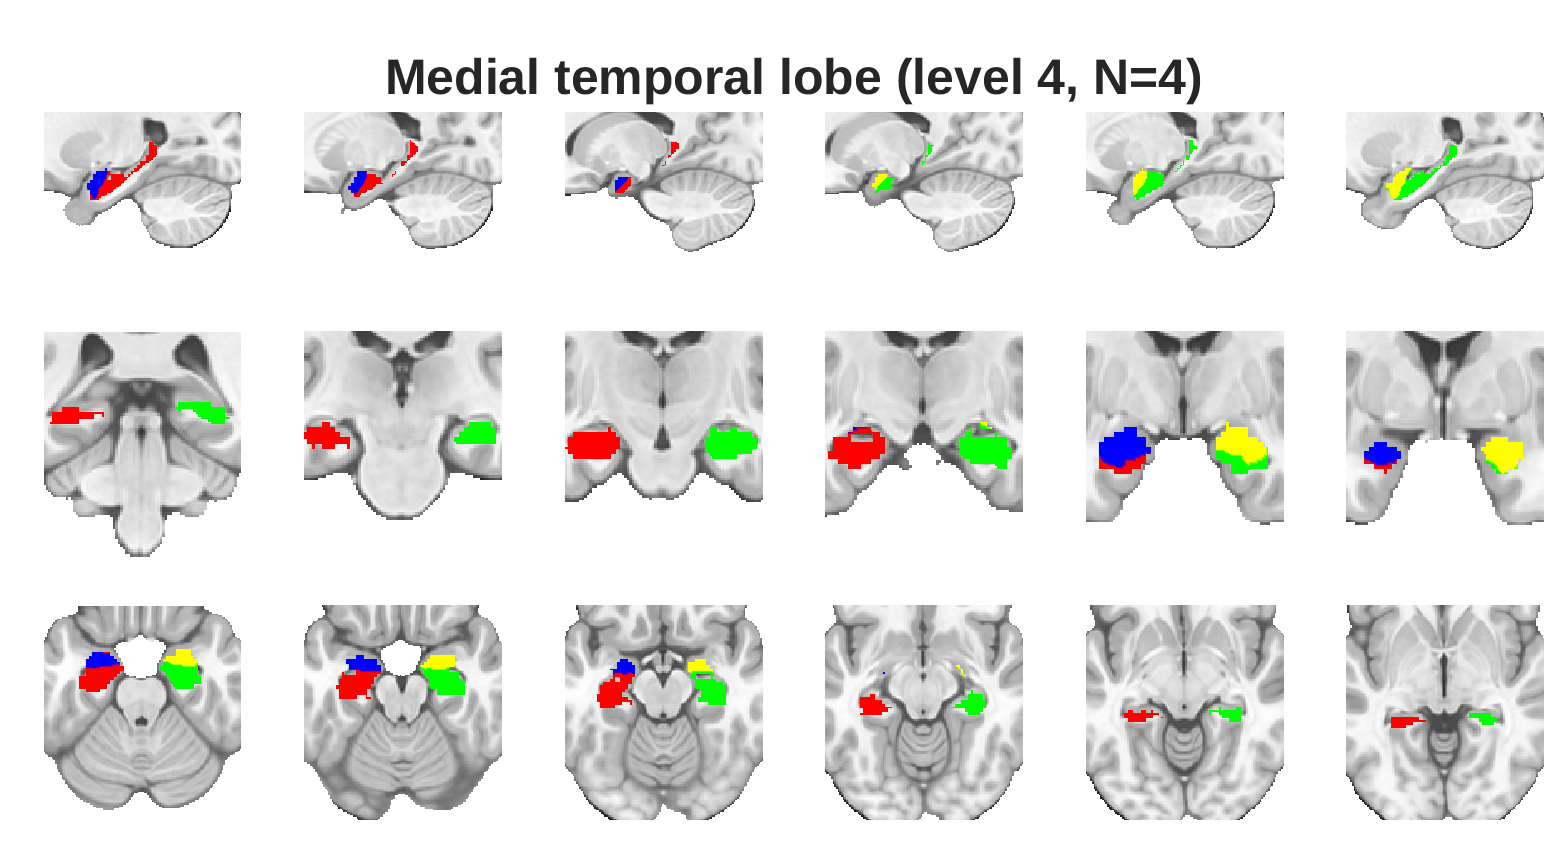
\includegraphics[width=\linewidth]{images/mtl_coarsest.png}
\end{minipage}
\caption{
{\bf
CANLab2024 Medial temporal lobe parcels.} At level 1 CANLab2024 distinguishes between intercalated nuclei of the amygdala, the central and median nuclei of the amygdala, and between CA2 and CA3 of the hippocampus. At level 2 these distinctions are collapsed and the intercallated nuclei are subsumed by their nearest neighbors while central and median nuclei and CA2 and CA3 are merged. A level 3 the amygdala is subdivided into basolateral, lateral and centromedian subdivisions, while the hippocampal formation is merely subdivided into hippocampus proper and subiculum. Level 4 subdivides the amygdala from the hippocampus.
}
\label{mtl-granularities-figure}
\end{figure}


\begin{figure*}[t!]
\centering
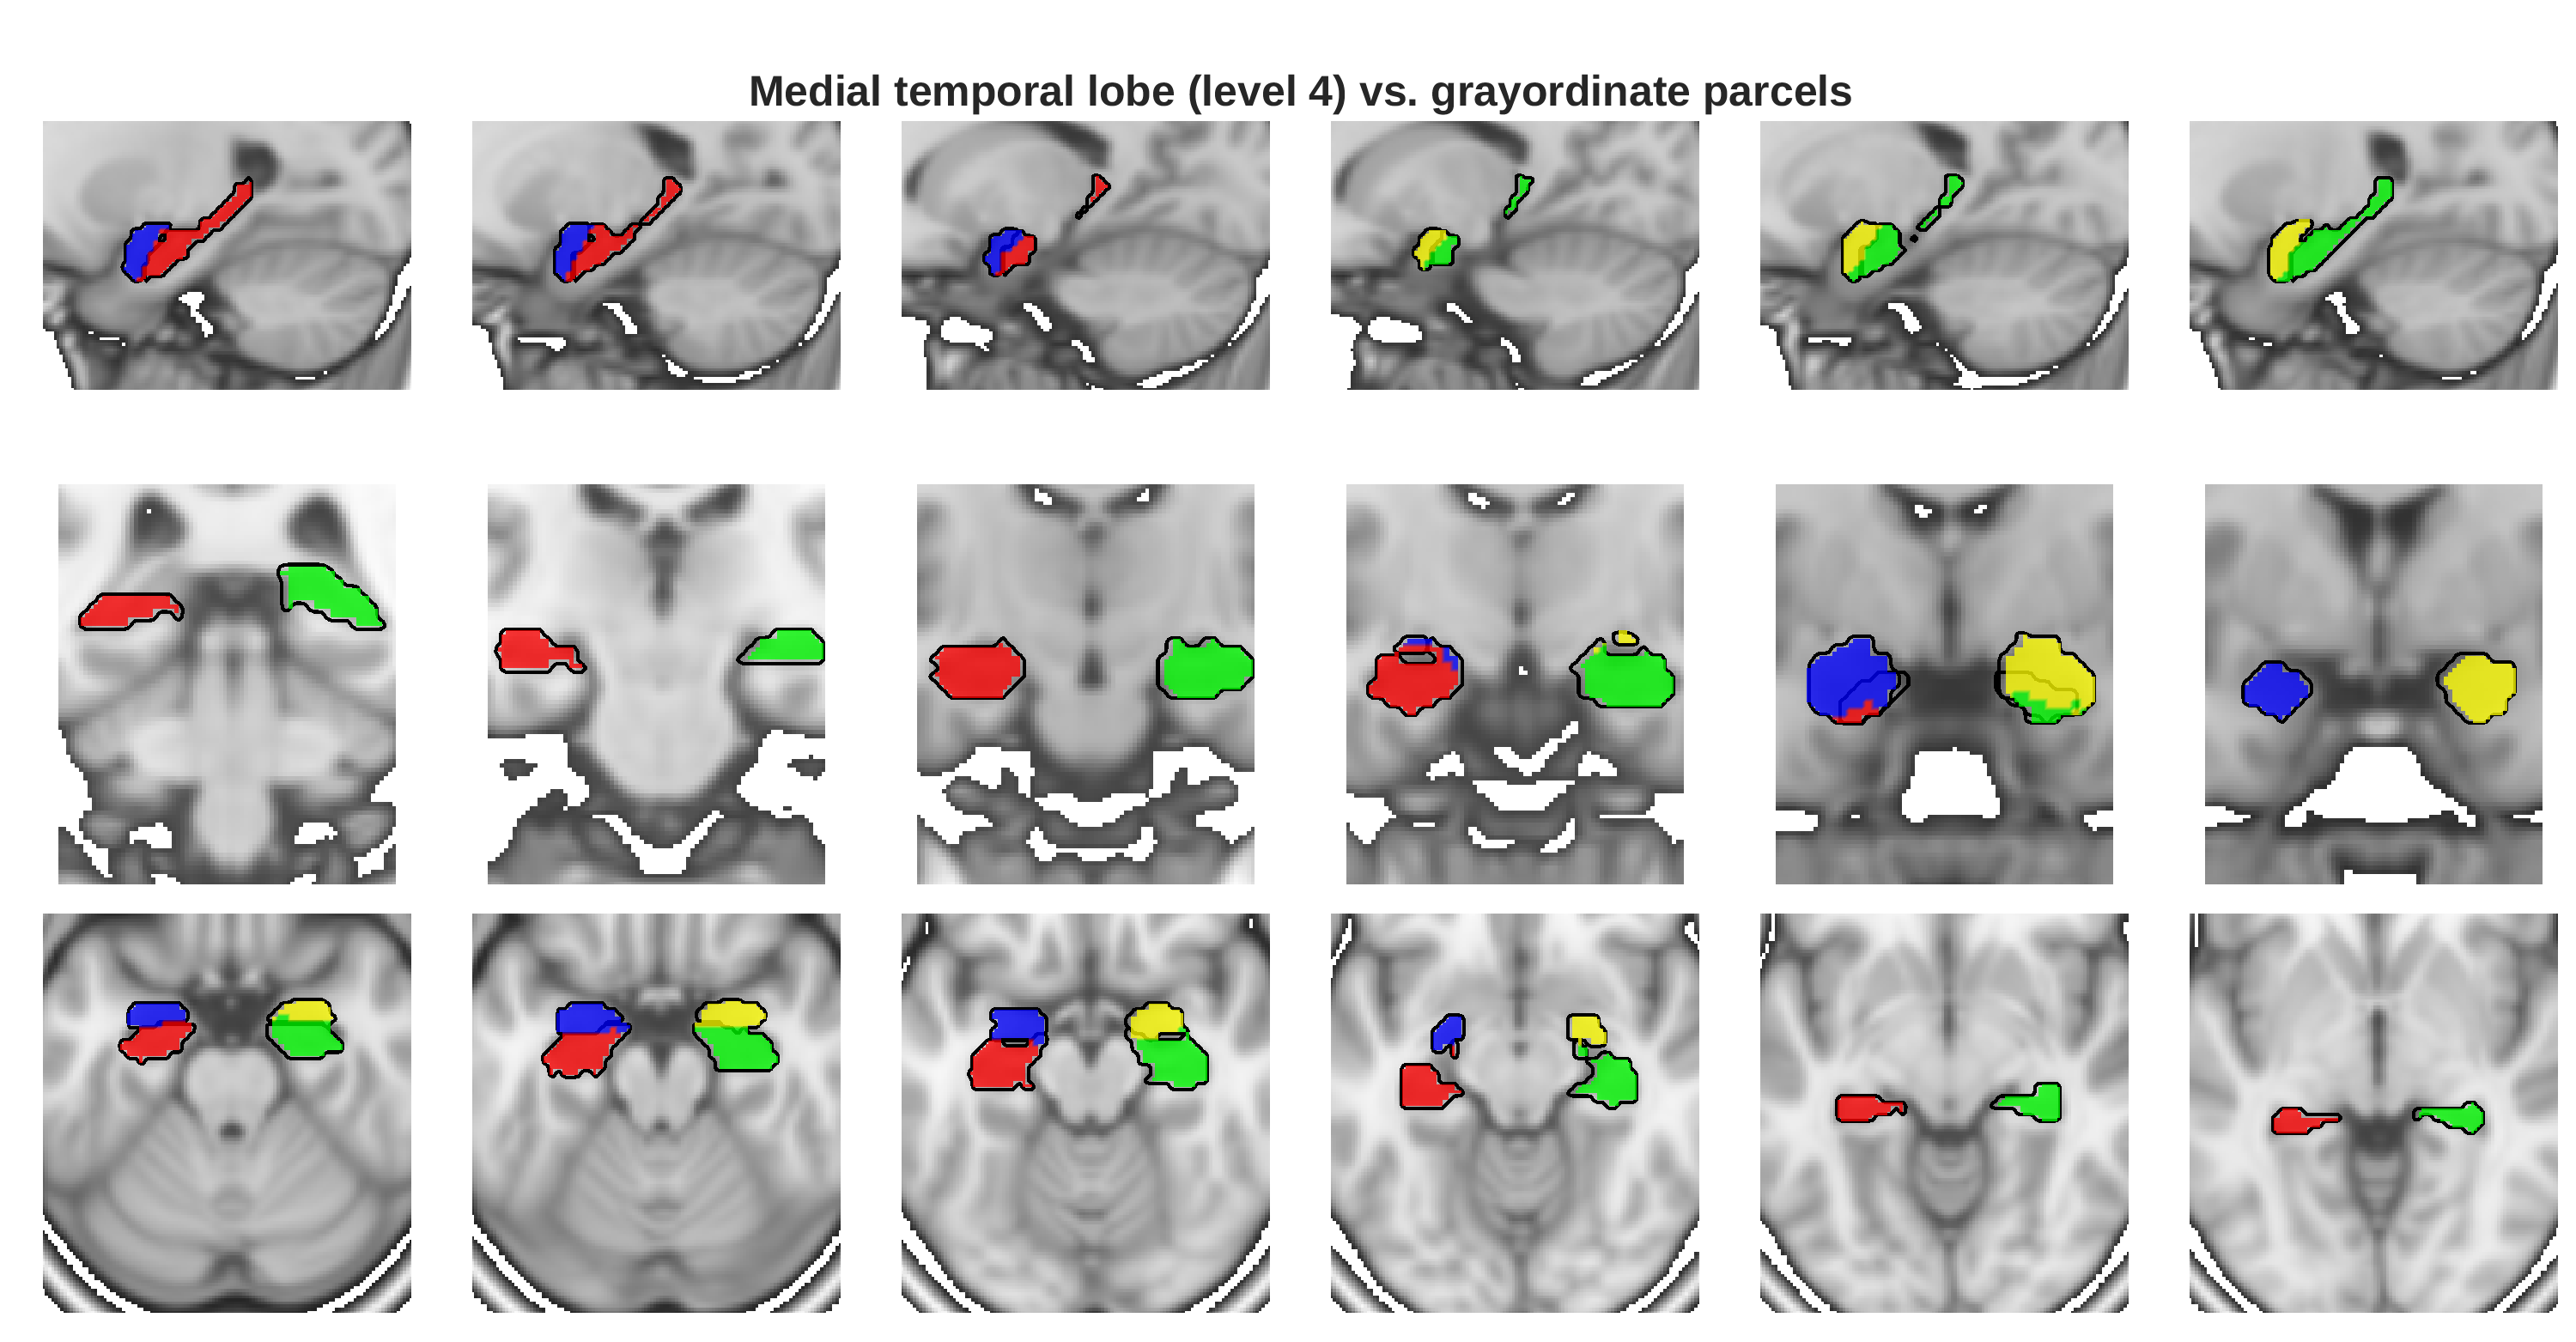
\includegraphics[width=\linewidth]{images/mtl_vs_cifti.png}
\caption{
{\bf
CANLab2024 medial temporal lobe parcels align well with HCP 91k grayordinate structural boundaries.} 
Colored outlines indicate the coarsest level of parcellation for the medial temporal lobe structures. Black lines illustrate the boundaries of HCP 91k grayordinate space. Underlay: MNI152NLin6Asym T1 2mm template, used by HCP 91k grayordinates.}
\label{mtl-vs-cifti-figure}
\end{figure*}

\subsubsection{Cerebellum} The cerebellar atlas is derived from the SUIT atlas \shortcite{Diedrichsen2009}. This parcellation was already quite coarse (Figure \ref{granularities-overview-figure}), distinguishing cerebellar lobules and segments of the vermis, so it was not downsampled further except for levels 3 and 4 of granularity (the coarsest two; Figure \ref{cblm-granularities-figure}).

\begin{figure}[t]
\centering
\begin{minipage}{\linewidth}
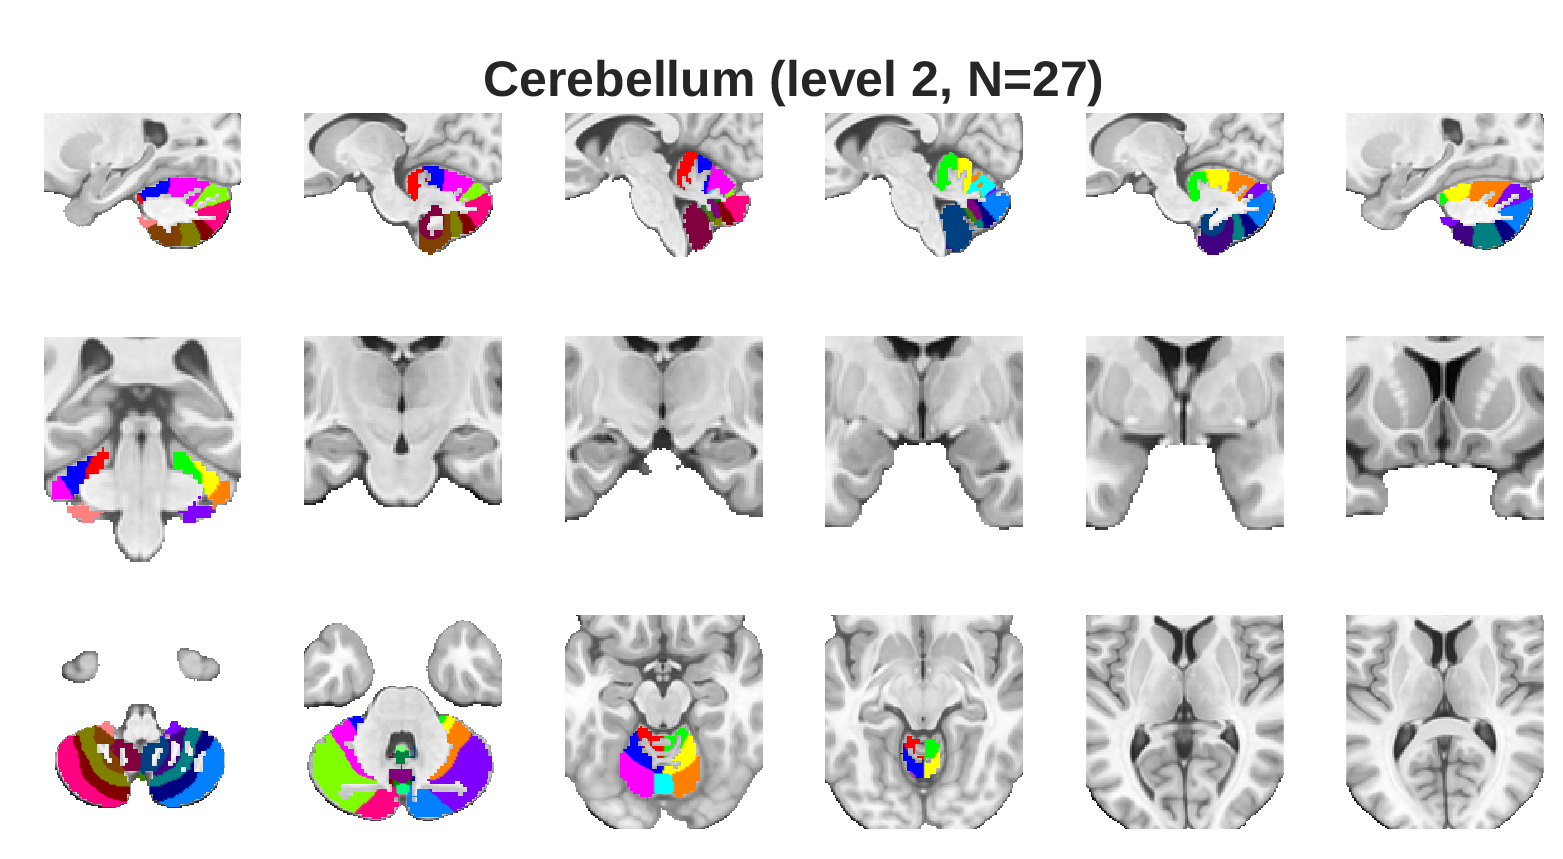
\includegraphics[width=\linewidth]{images/cblm_coarse.png}
\end{minipage}
\begin{minipage}{\linewidth}
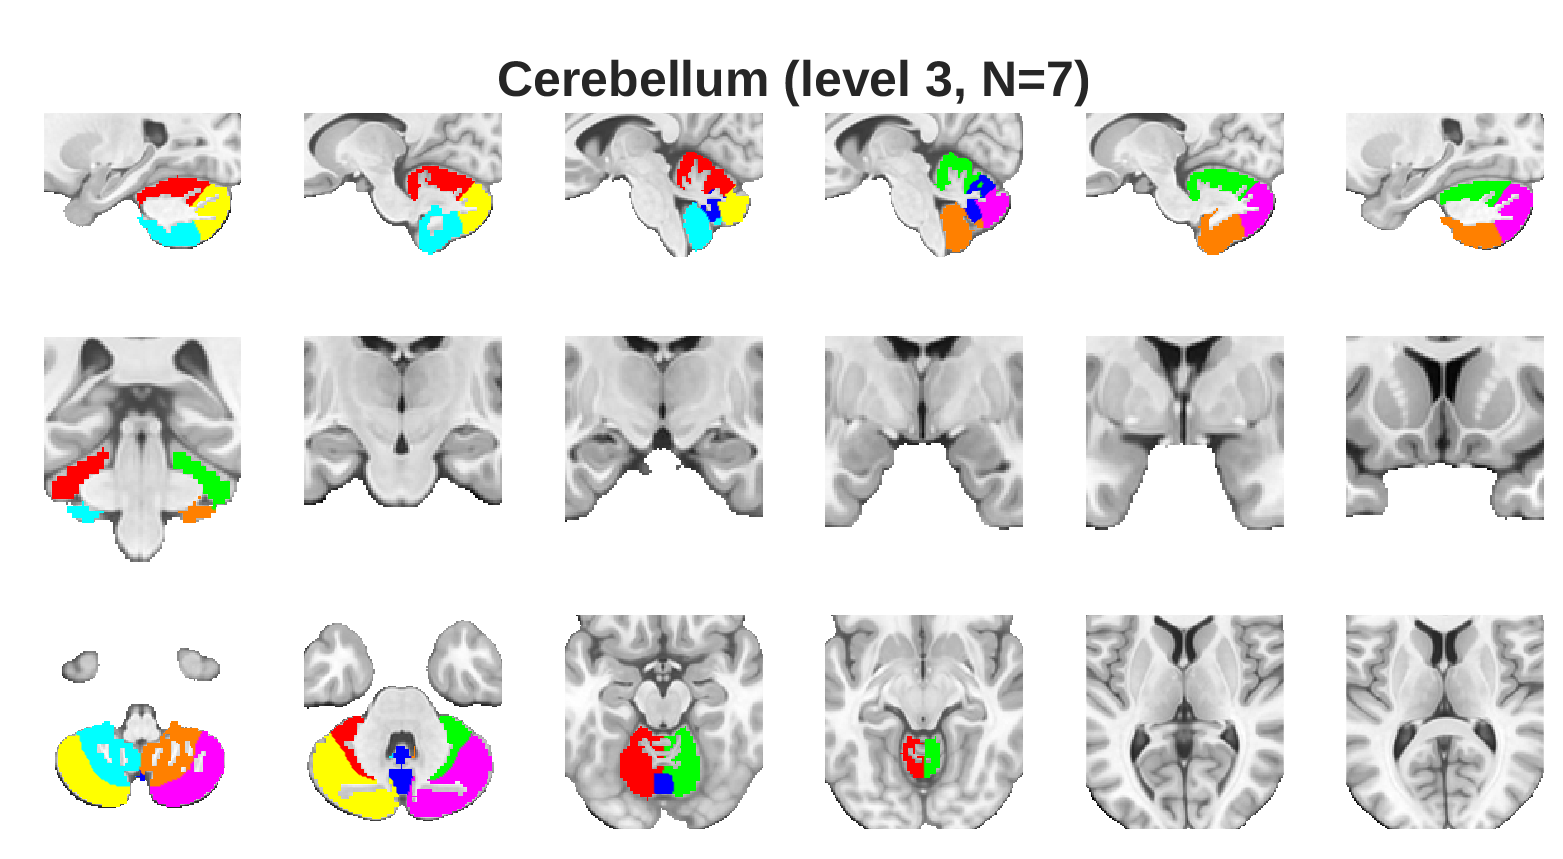
\includegraphics[width=\linewidth]{images/cblm_coarser.png}
\end{minipage}
\begin{minipage}{\linewidth}
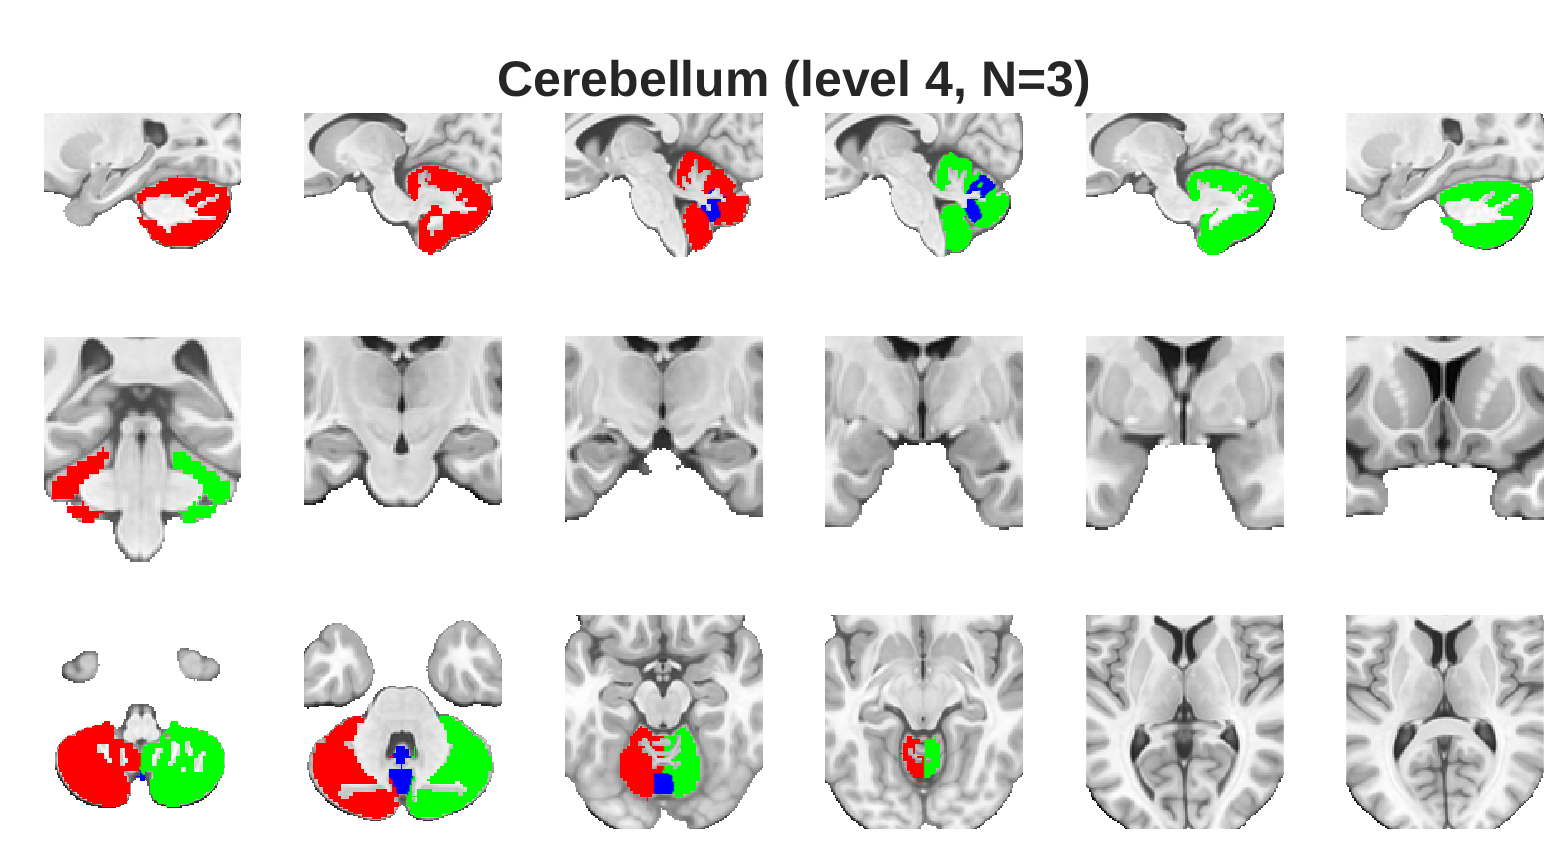
\includegraphics[width=\linewidth]{images/cblm_coarsest.png}
\end{minipage}
\caption{
{\bf
CANLab2024 cerebellar parcels.} Level 1 (not shown) is identical to level 2.
}
\label{cblm-granularities-figure}
\end{figure}

\subsubsection{Brainstem}


\begin{figure*}[t!]
\centering
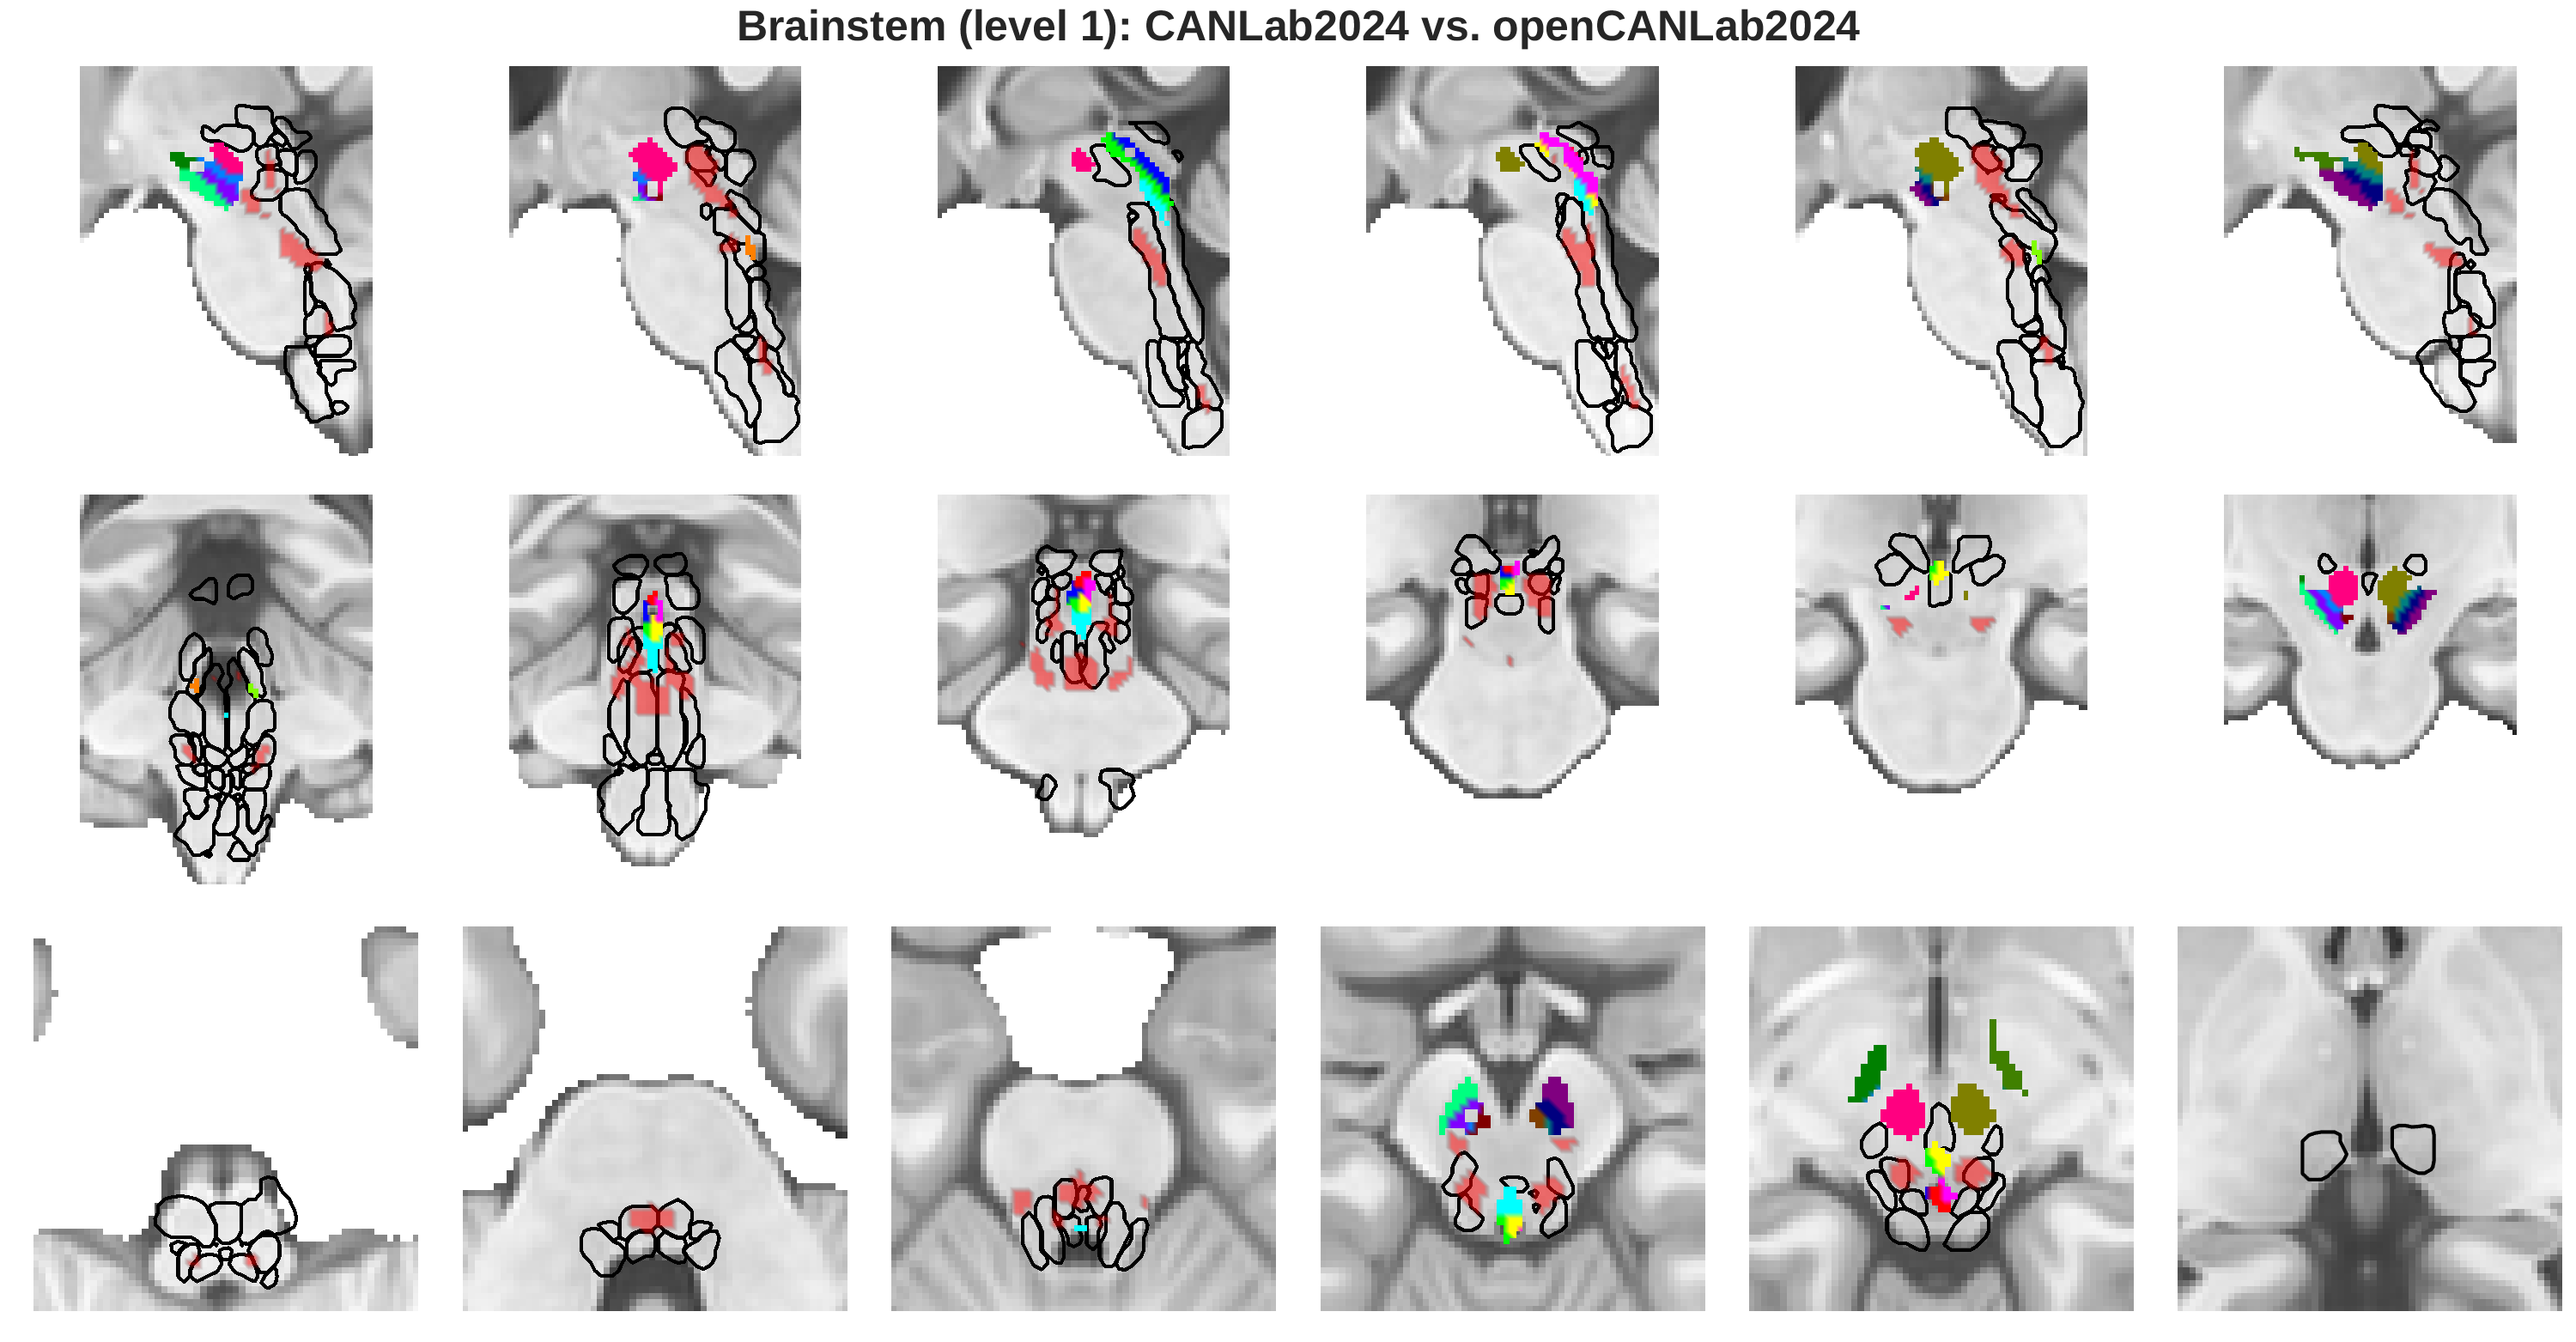
\includegraphics[width=\linewidth]{images/bstem_canlab_vs_opencanlab.png}
\caption{
{\bf
CANLab2024 differs from openCANLab2024 in the pons and medulla.} 
Openly licensed probablistic regions are largely shared between the two atlases (multicolored). CANLab2024 includes a number of regions with distribution restrictions (black outlines) and can only be incorporated into the copy of openCANLab2024 we distribute after being downloaded from a licensed repository. As a substitute we provide a number of pontine and medullary regions in openCANLab2024 (orange) that are non-probablistic, but have boundaries that roughly coincide with equivalent regions in CANLab2024. Finally, we provide a setup script which removes these regions, downloads the canlab2024 specific brainstem regions and inserts them appropriately to produce CANLab2024.}
\label{canlab2024-vs-opencanlab2024-bstem-figure}
\end{figure*}

\begin{figure}[t]
\centering
\begin{minipage}{\linewidth}
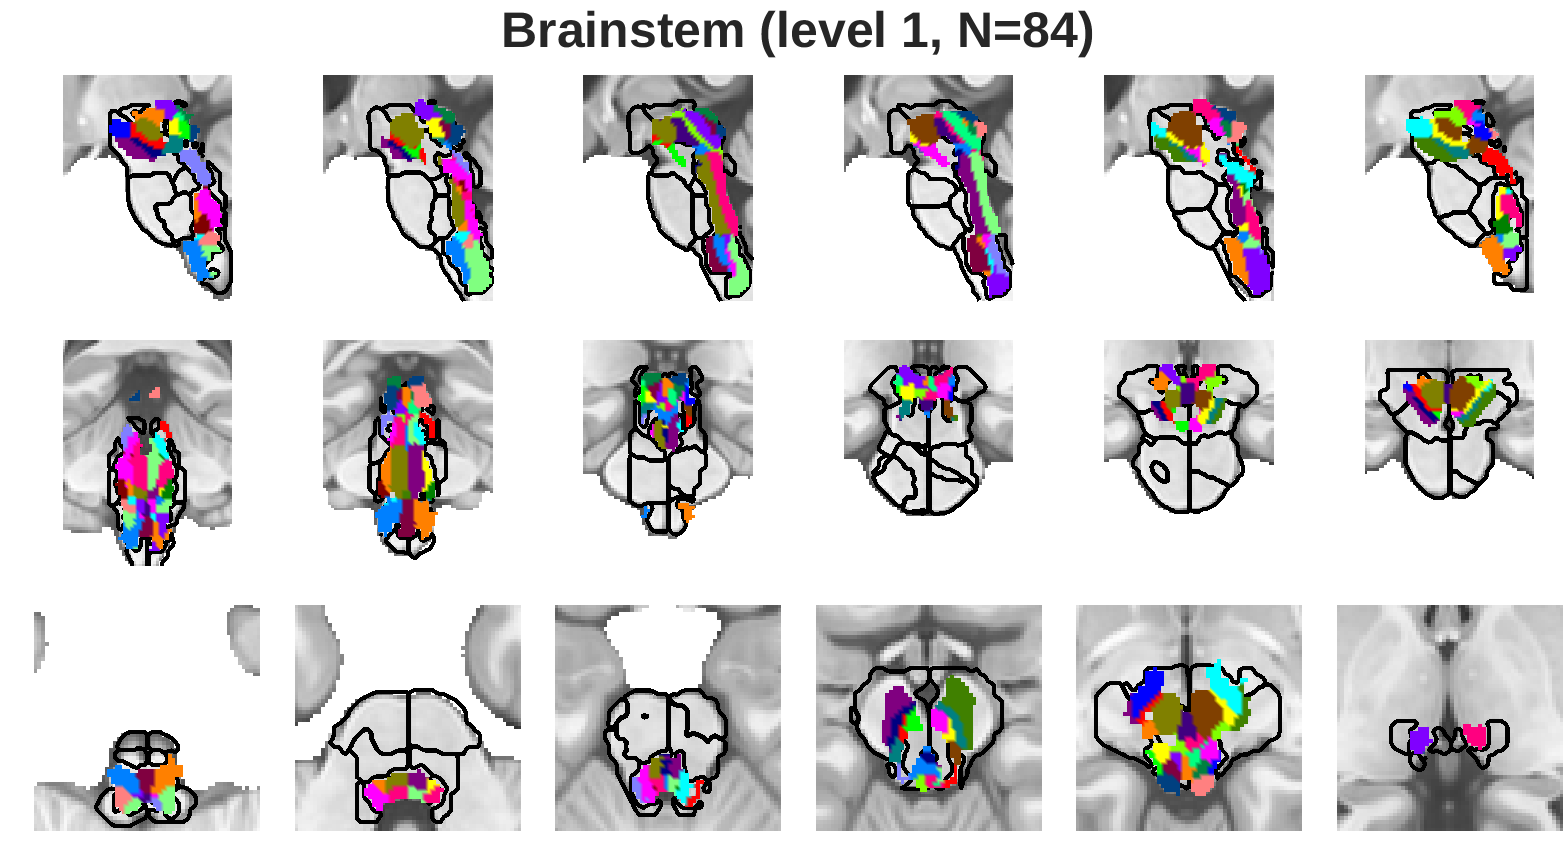
\includegraphics[width=\linewidth]{images/bstem_fine.png}
\end{minipage}
\begin{minipage}{\linewidth}
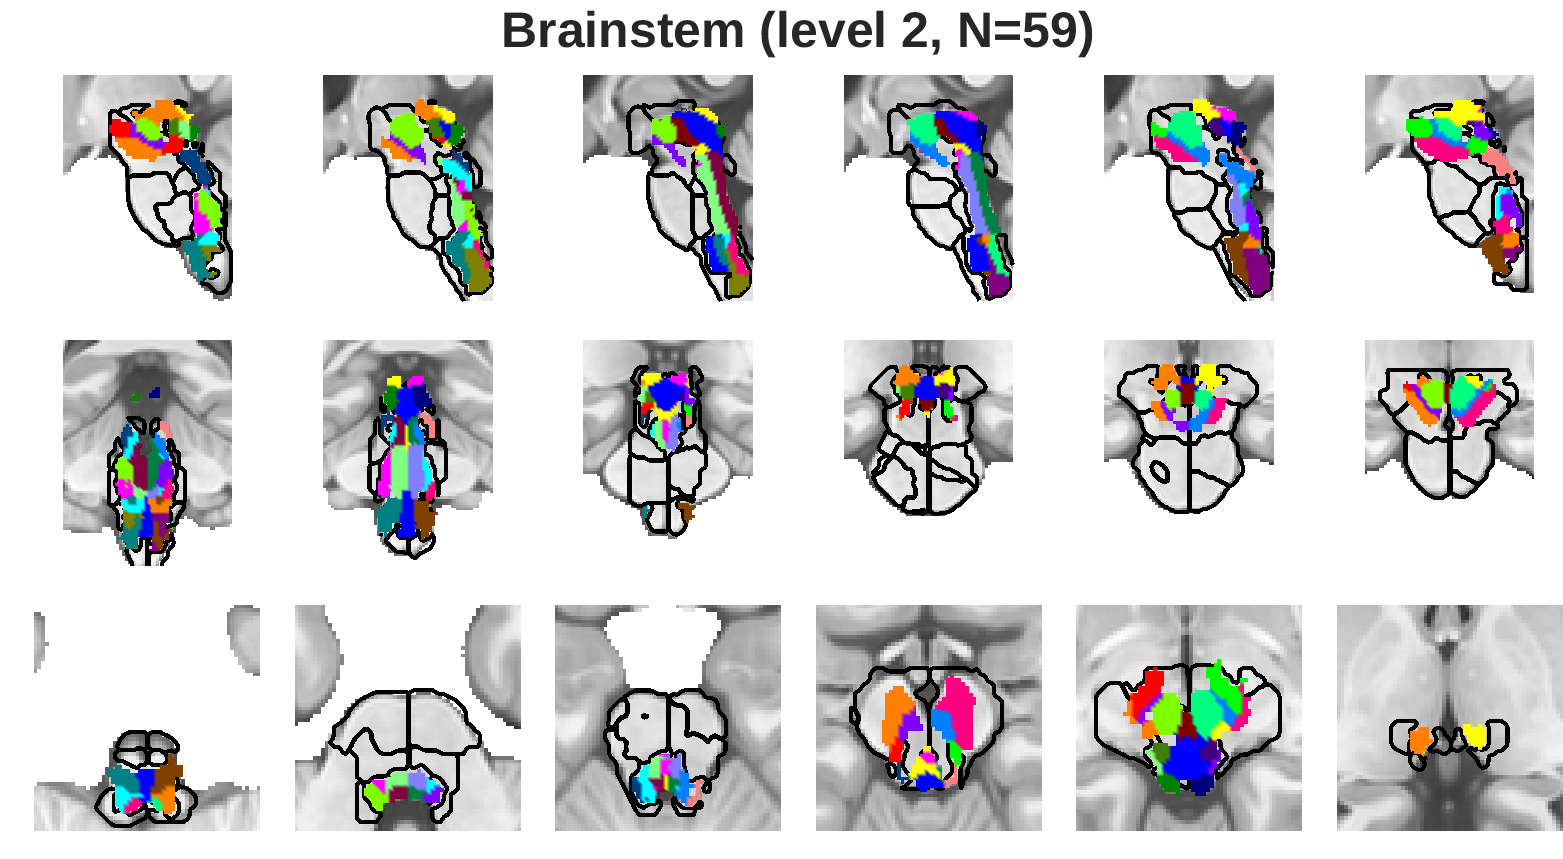
\includegraphics[width=\linewidth]{images/bstem_coarse.png}
\end{minipage}
\begin{minipage}{\linewidth}
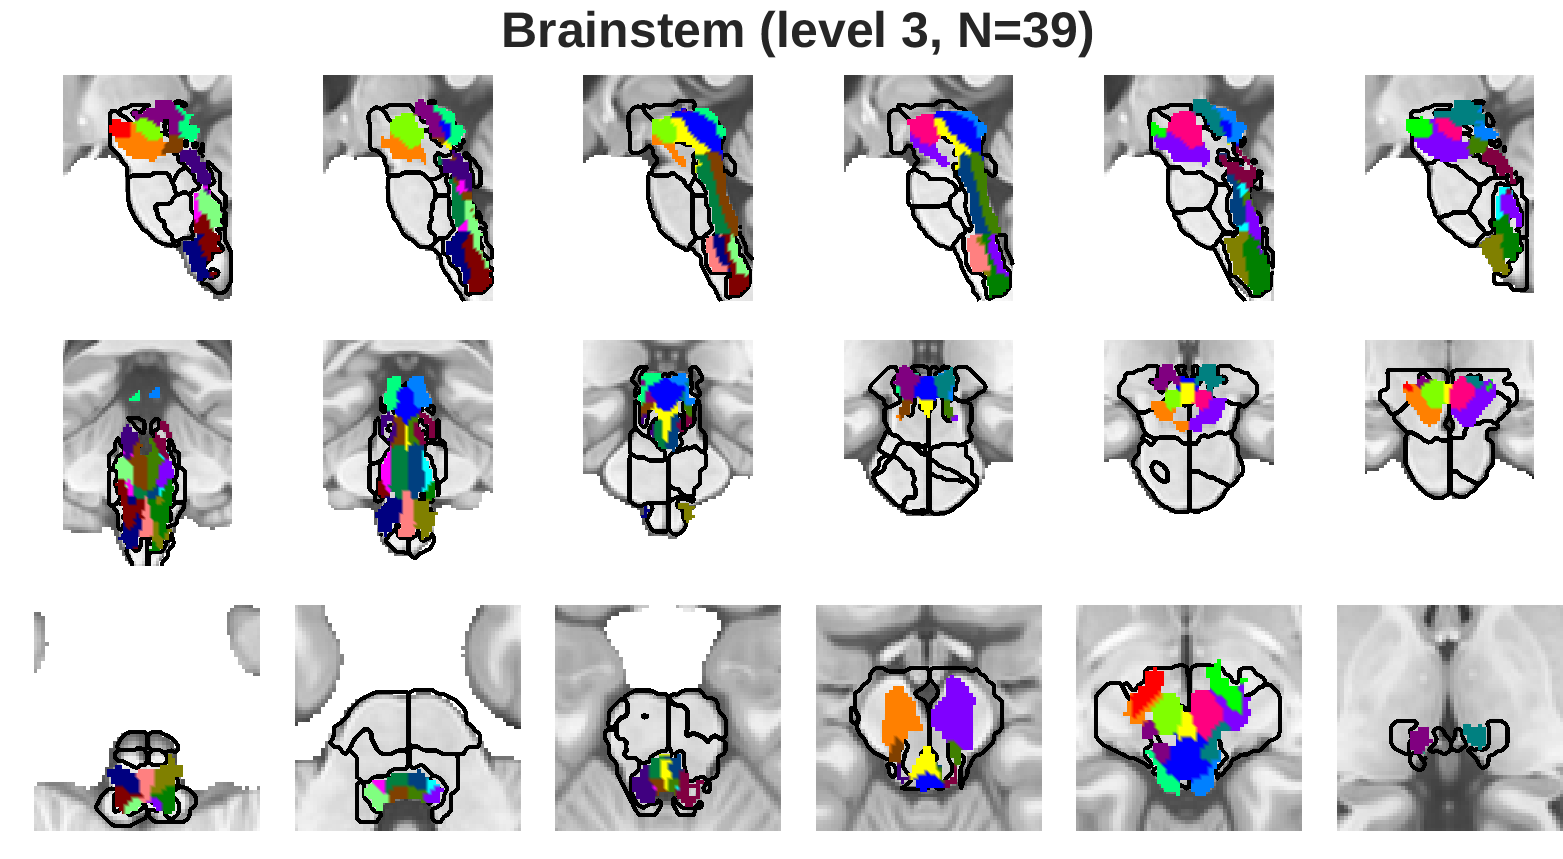
\includegraphics[width=\linewidth]{images/bstem_coarser.png}
\end{minipage}
\begin{minipage}{\linewidth}
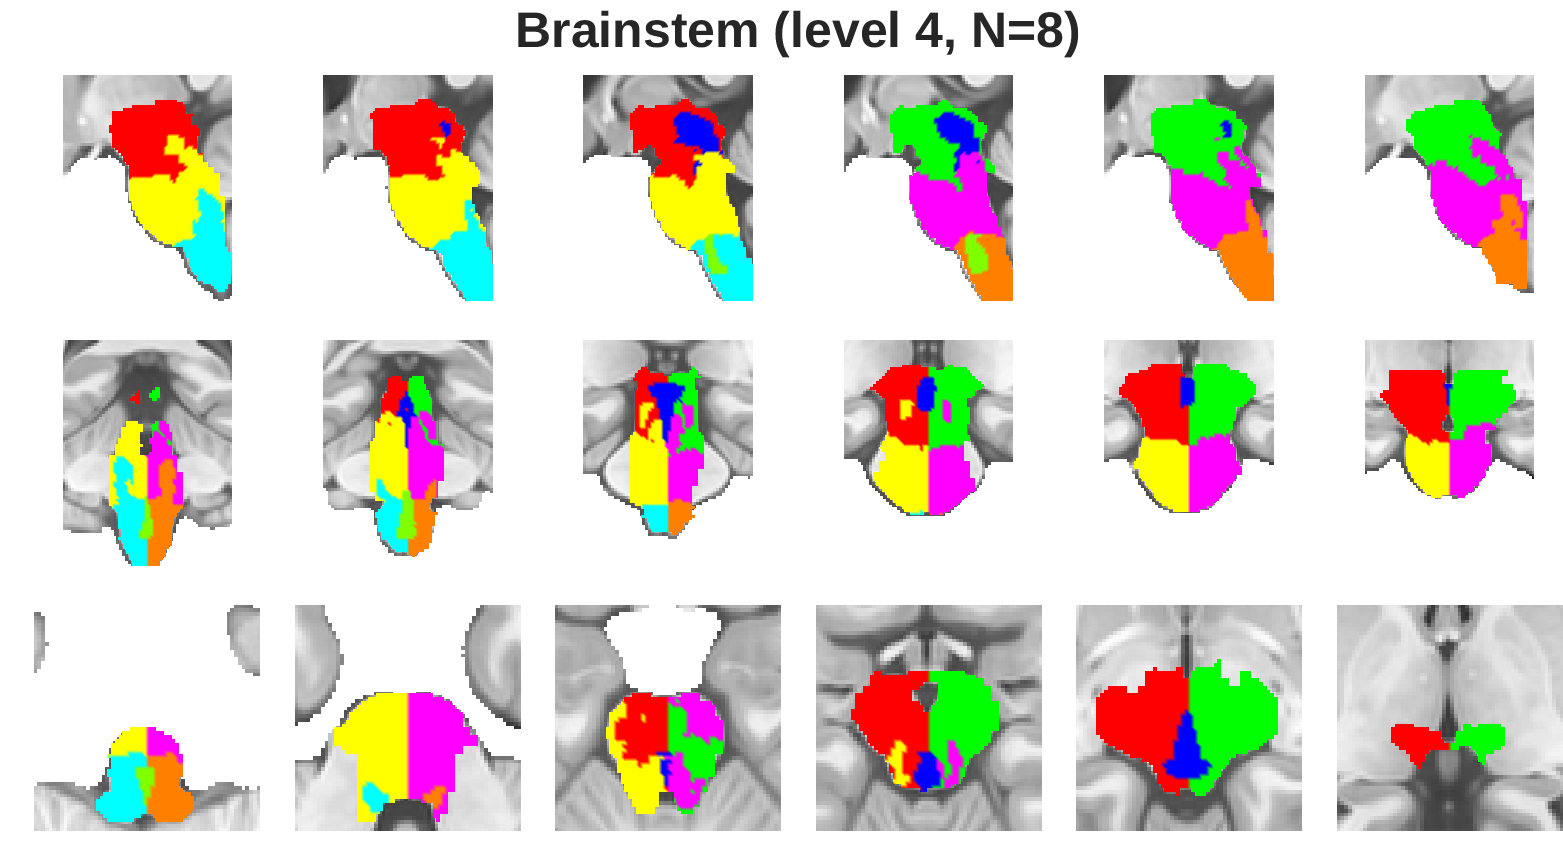
\includegraphics[width=\linewidth]{images/bstem_coarsest.png}
\end{minipage}
\caption{
{\bf
CANLab2024 brainstem parcels.} The brainstem is a mixture of highly intermingled gray and white matter structures, and not all gray matter structures are yet available in MNI coordinate digital atlases. To provide comprehensive coverage of the brainstem we combined available parcellations (colored) with filler regions defined by resting state functional network boundaries (black outlines). At the coarsest level of granularity these two divisions are merged.
}
\label{brainstem-granularities-figure}
\end{figure}

In the case of the brainstem we have gray matter and white matter intermingled, with poorly defined boundaries, and available digital atlases are incomplete. As a result we define the nuclei for which definitions are available but also introduce filler labels for residual voxels with descriptive labels (e.g. left ventral rostral pons). For display purposes we omit these latter regions. Additionally, the brainstem is where openCANLab2024 and CANLab2024 diverge due to the inclusion of regions from the Bianciardi brainstem atlas in the latter, which are not openly licensed. Thus, we focus here on highlighting these differences.

[This needs a plot of the level\_2 PAG vs. the level 1 PAG + CnF]

[compare locus coeruleus in Bianciardi and Levinson-Bari. Justify use of Levinson-Bari as similar enough and open]

[Could include neurotransmitter maps here potentially]


\section{Discussion}

[The difference in size of regions between cortex and cerebellum vs. brainstem, thalamus and BG should maybe not be surprising. The cortex and cerebellum are the two brain areas that had to fold in on themselves to be able to fit inside the skull. There's clearly something distinct about the scale at which they operate.]

\subsubsection{Cortex} Our volumetric cortical parcellation accounts for the idiosyncratic folding across individuals, but does not account for idiosyncracies in functional and structural topographies reported by Glasser et al. It seems unlikely at this point that Glasser et al. will ever release their idiosyncratic subject specific parcellations or the structural and functional feature based parcel classifiers they used to generate them, but their data is available and this leaves the door open for further refinements of this parcellation. Using the publicly available HCP data it would be possible to characterize each parcel in terms of population average multimodal features and use those to produce subject specific parcellations based on a nearest neighbor classification scheme or some similar strategy. It would be straightforward to combine such subject specific parcellations into probabilistic labels in surface space. Reprojection from surface to volume space would produce volumetric probabilistic labels that account for both area identity and its idiosyncratic embedding in 3D space. For now however our probabilities only account for idiosyncrasies in cortical folding, and should be used accordingly.

\subsubsection{Caudate/Putamen} [Address issues with using functional connectivity gradients as a criterion]

\subsubsection{Brainstem} [discuss how brainstem is incomplete and likely to continue to develop. Can give the RVM as an example region we tried to include but couldn't, and describe why we couldn't. Discuss licensing restrictions and alternative atlases (or the lack thereof). Discuss how localization is a problem here and how probablistic labels should be combined with expert knowledge to correctly attribute signals to structures. Can use the olivary complex as an example since SOC and ION are hard to distinguish. LC might be even better.]

\subsubsection{Variations across file formats}
[discuss the slight differences in the ventral striatum and hypothalamus, the absence of deep cerebellar nuclei, and the need for an update to the HCP 91k grayordinate template. Discuss surface representations of the cerebellum as well, and speculate on future extensions of the atlas that take advantage of superior grayordinate templates.]

\subsubsection{Credit attribution}
The efforts involved in assembling this atlas were substantial, but do no compare to those involved in generating the atlases we've built CANLab2024 from. We ask that those using CANLab2024 give credit where credit is due. Appropriate references are listed in Table \ref{constituent-atlas-table} for precisely this reason. This paper should be cited merely to the extent necessary for documenting our modifications to this prior work.


Limitations of histology? (registration issues, tissue distortion)

usefulness in neurosurgery?

what about still unlabeled voxels? Ideally we'd have a structural label for every single voxel. We still need white matter structures for this.


\section{Data Availability}
CANLab2024 and all constituent atlases are available online through our github repository: \url{https://github.com/canlab/Neuroimaging_Pattern_Masks/}. For further details regarding (open)CANLab2024 specifically please refer to \url{https://github.com/canlab/Neuroimaging_Pattern_Masks/tree/master/Atlases_and_parcellations/2024_CANLab_atlas/README.md}. All subject specific cortical projections used for registration fusion are available at \url{https://figshare.com/articles/dataset/2016_Glasser_MMP1_0_Cortical_Atlases/24431146}. 

\section{Acknowledgments}

We thank Ye Tian and Andrew Zalesky for sharing subject level segmentations of the basal ganglia, Henry Tregidgo and Juan Eugenio Iglesias for help with multimodal Bayesian segmentation of thalamic subnuclei, Philip A Kragel for suggesting the use of the CIT amygdala parcellation and providing subject specific PAG segmentations from which probabilities could be derived, and Mijin Kwon for guidance on optimal assignment of glasser parcels to the classic granular, agranular and dysgranular subdivisions of the insula.
\\
\\
This research was funded by NIBIB R01EB026549.

\bibliographystyle{apacite}

\setlength{\bibleftmargin}{.125in}
\setlength{\bibindent}{-\bibleftmargin}

\bibliography{references}

\end{document}
